\makeatletter
%\def\input@path{{../}}
\makeatother
\documentclass[main.tex]{subfiles}

\newcommand{\lfop}{\mathbf{L}_{\theta}}

\begin{document}
\section{Introduction}%
\label{sec:l2hmc_intro}
%
We describe a new technique for performing Hamiltonian Monte-Carlo (HMC) simulations called: `Learning to Hamiltonian
Monte Carlo' (L2HMC)~\cite{2017arXiv171109268L} which expands upon the traditional HMC by using a generalized version
of the leapfrog integrator that is parameterized by weights in a neural network.
%
In order to demonstrate the usefulness of this new approach, we use various metrics for measuring the performance of
the trained (L2HMC) sampler vs.\ the generic HMC sampler.
% how the trained (L2HMC) sampler performs
% compared to the generic HMC sampler.
%
First, we will look at applying this algorithm to a two-dimensional Gaussian Mixture Model (GMM).
%
The GMM is a notoriously difficult distribution for HMC due to the vanishingly small likelihood of the leapfrog
integrator traversing the space between the two modes.
%
Conversely, we see that through the use of a carefully chosen training procedure, the trained L2HMC sampler is able to
successfully discover the existence of both modes, and mixes (`tunnels') between the two with ease. 
% that for MCMC where it is observed that
% the trained sampler is able to successfully mix (`tunnel') between modes, while tthe HMC sampler is u
%
Additionally, we will observe that the trained L2HMC sampler mixes much faster than the generic HMC sampler, as
evidenced through their respective autocorrelation spectra.
%
This ability to reduce autocorrelations is an important metric for measuring the efficiency of a general MCMC
algorithm, and is of great importance for simulations in lattice gauge theory and lattice QCD.
%
Following this, we introduce the two-dimensional $U(1)$ lattice gauge theory and describe important modifications to
the algorithm that are of particular relevance for lattice models.
%
% Additionally, we see that the autocorrelation spectrum of the trained L2HMC sampler is a significant i
% significantly reduces autocorre
% We look at applying this technique to a two-dimensional Gaussian Mixture Model and a two-dimensional $U(1)$ lattice
% gauge theory, and compare our results against those obtained with traditional HMC. %chktex:13
%

%
Ongoing issues and potential areas for improvement are also discussed, particularly within the context of
high-performance computing and long-term goals of the lattice QCD community.
%
% L2HMC {{{
% \section{L2HMC}%
\section{Generalizing the Leapfrog Integrator}
% \label{sec:l2hmc_l2hmc}
As in the previously described HMC algorithm, we start by augmenting the current state $x \in \mathbb{R}^n$ with a
continuous momentum variable $v \in \mathbb{R}^{n}$ drawn from a standard normal distribution.
%
Additionally, we indtroduce a binary direction variable $d \in \{ -1, 1\}$, drawn from a uniform distribution. 
%
The complete augmented state is then denoted by $\xi \equiv (x, v, d)$, with probability density $p(\xi) = p(x) p(v)
p(d)$.
%
In order to improve the expressivity of our model, for each step $t$ of the leapfrog operator $\mathbf{L}_{\theta}$ we
assign a fixed random binary mask $m^{t} \in{\{0, 1\}}^n$ that will determine which variables are affected by each
sub-update.
%
The mask $m^t$ is drawn uniformly from the set of binary vectors satisfying $\sum_{i=1}^{n} m_{i}^{t} = \lfloor
\frac{n}{2}\rfloor$, i.e.\ half the entries of $m^t$ are $0$ and half are $1$.
%
Additionally, we write $\bar m^{t} = \mathbbm{1} - m^{t}$ and $x_{m^t} = x \odot m^{t}$, where $\odot$ denotes
element-wise multiplication, and $\mathbbm{1}$ the vector of $1$'s in each entry.
%
%
We begin with a subset of the augmented space, $\zeta_1 \equiv (x, \partial_{x} U(x), t)$, independent of the momentum
$v$.
%
We introduce three new functions of $\zeta_1$: $T_v$, $Q_v$, and $S_v$.
%
We can then perform a single time-step of our modified leapfrog integrator $\mathbf{L}_{\theta}$.
%

First, we update the momentum $v$, which depends only on the subset $\zeta_1$.
%
This update is written
%
\begin{equation}
  \vp = v \odot 
    \underbrace{\exp\left(\frac{\varepsilon}{2} S_{v}(\zeta_1)\right)}_{\text{\footnotesize{Momentum scaling}}}%
    - \frac{\varepsilon}{2}\left[\partial_{x} U(x)%
    \odot\underbrace{\exp(\varepsilon Q_{v}(\zeta_1))}_{\text{\footnotesize{Gradient scaling}}}%
    + \underbrace{T_v(\zeta_1)}_{\text{\footnotesize{Translation}}}\right].
    \label{eq:update_momentum_forward1}
\end{equation}
%
and the corresponding Jacobian is given by: $\exp{\left(\frac{\eps}{2}\mathbbm{1} \cdot S_{v}(\zeta_1)\right)}$.
%
Next, we update $x$ by first updating a subset of the coordinates of $x$ (determined according to the mask $m^t$),
followed by the complementary subset (determined from $\bar m^{t}$).
%
The first update affects only $x_{m^{t}}$ and produces $x^{\prime}$.
%
This update depends only on the subset $\zeta_2 \equiv (x_{\bar m^t}, v, t)$.
%
Following this, we perform the second update which only affects $x_{\bar{m}^t}^{\prime}$ and depends only on $\zeta_3
\equiv (x_{m^t}^{\prime}, v, t)$, to produce $x^{\prime\prime}$:
%
\begin{align}
  x^{\prime} &= x_{\bar{m}^t} + m^{t}\odot\left[x \odot \exp{(\eps S_x(\zeta_2))} + \eps\left(v^{\prime}\odot%
    \exp{(\eps Q_x(\zeta_2))} + T_x(\zeta_2)\right)\right]\\
  x^{\prime\prime} &= x^{\prime}_{m^t} + \bar m^t \odot \left[x^{\prime} \odot \exp{(\eps S_x(\zeta_3))} +%
    \eps\left(v^{\prime} \odot \exp{(\eps Q_x(\zeta_3))} + T_x(\zeta_3)\right)\right].
\end{align}
%
with Jacobians: $\exp{(\eps m^{t} \cdot S_x(\zeta_2))}$, and $\exp{(\eps \bar m^t \cdot S_x(\zeta_3))}$, respectively. 
%
Finally, we proceed to update $v$ again, using the subset $\zeta_4 \equiv (x^{\prime\prime}, \partial_{x}
U^{\prime\prime}, t)$: 
%
\begin{equation} 
  \vpp = \vp \odot \exp\left(\frac{\varepsilon}{2} S_v(\zeta_4)\right) - \frac{\varepsilon}{2}\left[\partial_{x} U
  \odot \exp(\varepsilon Q_v(\zeta_4)) + T_v(\zeta_4)\right].
    \label{eq:update_momentum_forward2}
\end{equation}
%
In order to build some intuition about each of these terms, we discuss below some of the subtleties contained in this
approach and how they are (carefully) dealt with.

The first thing to notice about these equations is that if $S_{i} = Q_{i} = T_{i} = 0$ ($i = x, v$), we recover the
previous equations for the generic leapfrog integrator (as we would expect since we are attempting to
\emph{generalize} HMC).
%
We can also see a similarity between the equations for updating $v$ and those for updating $x$: each update is
generalized by \emph{scaling} the previous value ($v$ or $x$), and \emph{scaling and translating} the updating
value (either $\partial_{x}\,U(x)$ or $x$).
%
It can be shown~\cite{2017arXiv171109268L}, that the scaling applied to the momentum in
Eq~\ref{eq:update_momentum_forward1} can enable, among other things, acceleration in low-density zones to facilitate
mixing between modes, and that the scaling term applied to the gradient may allow better conditioning of the energy
landscape (e.g., by learning a diagonal intertia tensor), or partial ignoring of the energy gradient for rapidly
oscillating energies.
%
Second, note that because the determinant of the Jacobian appears in the Metropolis-Hastings (MH) acceptance
probability, we require the Jacobian of each update to be efficiently computable (i.e.\ independent of the variable
actually being updated).
%
For each of the momentum updates, the input is a subset $\zeta = (x, \partial_{x}\,U(x), t)$ of the augmented space and
the associated Jacobian is $\exp{\left(\frac{\eps}{2}\mathbbm{1}\cdot S_{v}(\zeta)\right)}$ which is independent of $v$
as desired.
%
For the position updates however, things are complicated by the fact that the input $\zeta$ is $x$-dependent.
%
In order to ensure that the Jacobian of the $x$ update is efficiently computable, it is necessary to break the update
into two parts following the approach outlined in \emph{Real-valued Non-Volume Preserving transformations
(RealNVP)}~\cite{dinhRealNVP}.

%
% \subsection{MCMC Transitions}
\subsection{Metropolis-Hastings Accept/Reject}
%
Written in terms of these transformations, the augmented leapfrog operator $\mathbf{L}_{\theta}$ consists of $M$
sequential applications of the single-step leapfrog operator $\mathbf{L}_{\theta} \xi = \mathbf{L}_{\theta}(x, v, d) =
(x^{\prime\prime\times M}, v^{\prime\prime\times M}, d)$, followed by the previously-defined momentum flip operator
$\mathbf{F}$ which flips the direction variable $d$, i.e.\ $\mathbf{F}\xi = (x, v, -d)$.
%
Using these, we can express a complete molecular dynamics update step as $\mathbf{FL}_{\theta}\xi = \xip$, where now
the Metropolis-Hastings acceptance probability for this proposal is given by
%
\begin{equation}
    A(\mathbf{F}\mathbf{L} \xi | \xi) = \min\left(1,
        \frac{p(\mathbf{F}\mathbf{L}\xi)}{p(\xi)}\left|
        \frac{\partial\left[\mathbf{F}\mathbf{L}\xi\right]}
            {\partial\xi^{T}}\right|\right),
\end{equation}
%
Where $\left|\frac{\partial\left[\mathbf{F}\mathbf{L}\xi\right]} {\partial\xi^{T}}\right|$ denotes the determinant of
the Jacobian describing the transformation.

In contrast to generic HMC where $\left|\frac{\partial\left[\mathbf{F}\mathbf{L}\xi\right]} {\partial\xi^{T}}\right| =
1$, we now have non-symplectic transformations (i.e.\ non-volume preserving) and so we must explicitly account for the
determinant of the Jacobian.
%
These non-volume preserving transformations have the effect of deforming the energy landscape, which, depending on the
nature of the transformation, may allow for the exploration of regions of space which were previously inaccessible.
%
\newcommand{\energyA}{\includegraphics[width=0.4\textwidth]{energy_landscape/original_energy_landscape.pdf}}
\newcommand{\energyB}{\includegraphics[width=0.4\textwidth]{energy_landscape/modified_energy_landscape.pdf}}
%
\begin{figure}
  \centering 
  \Huge
  \parbox{\widthof{\energyA}}{\energyA} $\overset{\mathcal{J}}{\longrightarrow}$
  \parbox{\widthof{\energyB}}{\energyB} 
  \normalsize
  \caption{Example of how the determinant of the Jacobian can deform the energy landscape.}
\end{figure}


% \[\vcenter{\energyA} \hbox{\Huge\overset{\mathcal{J}}{\longrightarrow}} \vcenter{\energyB}\]
% \begin{figure}[htpb]
%     \centering
%     \vcenter{
%     \includegraphics[width=0.4\textwidth]{energy_landscape/original_energy_landscape.pdf}
%     \Huge$\overset{\mathcal{J}}{\longrightarrow}$
%     % \includegraphics[width=0.15\texwidth]{energy_landscape/jacobian1.pdf}
%     \includegraphics[width=0.4\textwidth]{energy_landscape/modified_energy_landscape.pdf}
%     \caption{Example of how the determinant of the Jacobian can deform the
%       energy landscape. (left) Molecular dynamics (MD) update gets stuck in
%       one of the two local minima. (right) After deforming the energy
%       landscape, the MD update is able to explore both minima, resulting in a
%       better description of the target
%       distribution.}\label{fig:energy_barrier}
% \end{figure}
%
To simplify our notation, introduce an additional operator $\mathbf{R}$ that re-samples the momentum and direction,
e.g.\ given $\xi = (x, v, d)$, $\mathbf{R}\,\xi = (x, v^{\prime}, d^{\prime})$ where $v^{\prime} \sim \mathcal{N}(0,
I)$, $d^{\prime} \sim \mathcal{U}\left(\{-1, 1\}\right)$.
%
A complete sampling step of our algorithm then consists of the following two steps:
%
\begin{enumerate}
    \item $\xi^{\prime} = \mathbf{FL}_{\theta} \,\xi$ with probability
        $A(\mathbf{FL}_{\theta}\,\xi|\xi)$ (Eq.~\ref{eq:metropolis_hastings}),
        otherwise $\xi^{\prime} = \xi$.
    \item $\xi^{\prime} = \mathbf{R}\,\xi$.
\end{enumerate}
%
Note however, that for MH to be well-defined, this deterministic operator must be \emph{invertible} and \emph{have a
tractable Jacobian} (i.e.\ we can compute its determinant).
%
In order to make this operator invertible, we augment the state space $(x, v)$ into $(x, v, d)$, where $d \in \{-1,
1\}$ is drawn with equal probability and represent the direction of the update.
%
All of the previous expressions for the augmented leapfrog updates represent the forward ($d = 1$) direction.
%
We can derive the expressions for the backward direction ($d = -1$) by reversing the order of the updates (i.e.\ $\vpp
\rightarrow \vp$, then $\xpp \rightarrow \xp$, followed by $\xp \rightarrow x$ and finally $\vp \rightarrow v$).
%
For completeness, we include in Sec.~\ref{sec:lf_forward} and
Sec~\ref{sec:lf_backward} all of the equations (both forward and backward directions)
relevant for updating the variables of interest in our augmented leapfrog sampler.

%
% \clearpage
% \subsection{Augmented Leapfrog Equations}%
% \label{subsec:augmented_leapfrog_equations}
%
\section{Forward direction \texorpdfstring{$(d = 1)$}{(d = 1)}:}%
\label{sec:lf_forward}
% \vspace{-20pt}
\begin{align}
  \vp &= v \odot \exp{\left(\frac{\eps}{2}S_{v}(\zeta_{1})\right)}% 
        - \frac{\eps}{2}\left[\partial_{x}\,U(x)\odot \exp{\left(\eps Q_{v}(\zeta_{1})\right)}%
        + T_{v}(\zeta_{1})\right] \\
  \xp &= x_{\bar{m}^{t}} + m^{t}\odot \left[x \odot \exp{\left(\eps S_{x}(\zeta_{2})\right)}%
        + \eps\left(\vp\odot\exp{\left(\eps Q_{x}(\zeta_{2})\right)} + T_{x}(\zeta_{2})\right)\right] \\
  \xpp &= x^{\prime}_{m^{t}} + \bar{m}^{t}\odot \left[\xp \odot \exp{\left(\eps S_{x}(\zeta_{3})\right)}%
        + \eps\left(\vp\odot\exp{\left(\eps Q_{x}(\zeta_{3})\right)} + T_{x}(\zeta_{3})\right)\right] \\
  \vpp &= \vp \odot \exp{\left(\frac{\eps}{2}S_{v}(\zeta_{4})\right)}%
        - \frac{\eps}{2}\left[\partial_{x}\,U(\xpp)\odot \exp{\left(\eps Q_{v}(\zeta_{4})\right)}%
          + T_{v}(\zeta_{4})\right]
\end{align} 
%
With $\zeta_{1} = (x, \partial_{x}\, U(x), t)$, $\zeta_{2} = (x_{\bar{m}^{t}}, v, t)$, $\zeta_{3} =
(x^{\prime}_{m^{t}}, v, t)$, $\zeta_{4} = (\xpp, \partial_{x}\, U(\xpp), t)$.
%
\section{Backward direction \texorpdfstring{$(d = -1)$}{(d = -1)}:}%
\label{sec:lf_backward}
%
\begin{align}
  v^{\prime} &= {\left\{v + \frac{\eps}{2}\left[\partial_{x}\,U(x)\odot \exp{\left(\eps Q_{v}(\zeta_{1})\right)}%
    + T_{v}(\zeta_{1})\right]\right\}} \odot \exp{\left(-\frac{\eps}{2}S_{v}(\zeta_{1})\right)} \\
  \xp &= x_{m^{t}} + \bar{m}^{t}\odot%
    {\left[x - \eps{\left(\exp{\left(\eps Q_{x}(\zeta_{2})\right)}\odot \vp%
    + T_{x}(\zeta_{2})\right)}\right]}\odot \exp{\left(-\eps S_{x}(\zeta_{2})\right)} \\
  \xpp &= x_{\bar{m}^{t}} + m^{t}\odot%
    {\left[\xp - \eps{\left(\exp{\left(\eps Q_{x}(\zeta_{3})\right)}\odot \vp%
    + T_{x}(\zeta_{3})\right)}\right]}\odot \exp{\left(-\eps S_{x}(\zeta_{3})\right)} \\
  v^{\prime\prime} &= {\left\{\vp + \frac{\eps}{2}\left[\partial_{x}\,U(\xpp)\odot%
    \exp{\left(\eps Q_{v}(\zeta_{1})\right)}
    + T_{v}(\zeta_{1})\right]\right\}}\odot 
    \exp{\left(-\frac{\eps}{2}S_{v}(\zeta_{4})\right)}
\end{align}
%
With $\zeta_{1} = (x, \partial_{x}\, U(x), t)$, $\zeta_{2} = (x_{m^{t}}, v, t)$, $\zeta_{3} =
(x^{\prime}_{\bar{m}^{t}}, v, t)$, $\zeta_{4} = (\xpp, \partial_{x}\, U(\xpp), t)$.
%
\section{Determinant of the Jacobian}
In terms of the auxiliary functions $S_{i}, Q_{i}, T_{i}$, we can compute the Jacobian:
%
\begin{align}
  \log|\mathcal{J}| 
  &= \log\bigg|\frac{\partial{\left[\mathbf{FL}_{\theta}\xi\right]}}{\partial \xi^{T}}\bigg|\\
  &= d \sum_{t\leq N_{\mathrm{LF}}}
    {\left[\frac{\eps}{2} \mathbbm{1}\cdot S_{v}(\zeta_{1}^{t}) + \eps m^{t} \cdot S_{x}(\zeta_{2}^{t}) 
      + \eps \bar{m}^{t} \cdot S_{x}(\zeta_{3}^{t}) + \frac{\eps}{2}\mathbbm{1} \cdot S_{v}(\zeta_{4}^{t})\right]}.
\end{align}
%
where $N_{\mathrm{LF}}$ is the number of leapfrog steps, and $\zeta_{i}^{t}$ denotes the intermediary variable
$\zeta_{i}^{t}$ at time step $t$ and $d$ is the direction of $\xi$, i.e.\ $d = 1 \,\, (-1)$ for the forward (backward)
update.
%
\section{Network Architecture}%
\label{subsec:l2hmc_network}
As previously mentioned, each of the functions $Q$, $S$, and $T$, are implemented using multi-layer perceptrons with
shared weights.
%
It's important to note that we keep separate the network responsible for paramterizing the functions used in the
position updates (`$\Xnet$', i.e.\ $Q_x$, $S_x$, and $T_x$), and the network responsible for parameterizing the
momentum updates (`$\Vnet$', i.e.\ $Q_v$, $S_v$, and $T_v$).
%
Since both networks are identical, we describe the architecture of $\Vnet$ below, and include a flowchart for $\Xnet$ 
illustrative purposes in Fig~\ref{fig:x_net_flowchart}.
%
%
\begin{figure}[htpb]
  \centering
  \includegraphics[width=\textwidth]{generic_net/generic_net4.png}
  \caption{Illustration showing the generic (fully-connected) network architecture for training $S_v$, $Q_v$, and
  $T_v$.}%
\label{fig:generic_net}
\end{figure}
%
%
% Each of these networks have identical architectures, and without loss of generality we describe the architecture of the
% position network below.
%
% Since the networks responsible for updating the, we describe the network architecture responsible for updating the
% momentum $v$.

The network takes as input $\zeta_1 = (x, \partial_{x} U(x), t)$, where $x, v \in \mathbb{R}^{n}$, and $t$ is encoded
as $\tau(t) = \left(\cos{(\frac{2\pi t}{N_{\mathrm{LF}}})},\right.  \left.\sin{(\frac{2\pi
t}{N_{\mathrm{LF}}})}\right)$.
%
Each of the inputs is then passed through a fully-connected (`dense' layer), consisting of $n_h$ hidden units
%
\begin{align}
    \tilde x &= W^{(x)} x + b^{(x)} \quad (\in \mathbb{R}^{n_h})\\
    \tilde v &= W^{(v)} v + b^{(v)} \quad (\in \mathbb{R}^{n_h})\\
    \tilde \tau &= W^{(\tau)} \tau + b^{(\tau)} \quad (\in \mathbb{R}^{n_h}).
\end{align}
%
Where $W^{(x)}, W^{(v)} \in \mathbb{R}^{n \times n_h}$, $W^{(t)} \in \mathbb{R}^{2 \times n_h}$, and $b^{(x)}$,
$b^{(v)}$,  $b^{(t)} \in \mathbb{R}^{n_h}$.
%
From these, the network computes
%
\begin{equation}
    h_1 = \sigma(\tilde x + \tilde v + \tilde \tau) \quad (\in
    \mathbb{R}^{n_h}).
    \label{eq:hidden_1}
\end{equation}
%
Where $\sigma(x) = \max(0, x)$ denotes the rectified linear unit (ReLU) activation function.
%
Next, the network computes
%
\begin{equation}
    h_2 = \sigma\left(W^{(h_1)} h_1 + b^{(h_1)}\right) \quad (\in
    \mathbb{R}^{n_h}).
    \label{eq:hidden_2}
\end{equation}
%
These weights ($h_2$) are then used to compute the network's output:
%
\begin{align}
    S_x &= \lambda_s \tanh(W^{(s)} h_2 + b^{(s)})\quad (\in \mathbb{R}^{n})\\
    Q_x &= \lambda_q \tanh(W^{(q)} h_2 + b^{(q)})\quad (\in \mathbb{R}^{n})\\
    T_x &= W^{(T)} h_2 + b^{(T)}\quad (\in \mathbb{R}^{n}),
\end{align}
%
Where $W^{(s)}, W^{(q)}$, and $W^{(T)} \in \mathbb{R}^{n_h \times n}$ and $b^{(s)}, b^{(q)}$, and $b^{(T)} \in
\mathbb{R}^{n}$.
%
The parameters $\lambda_s$ and $\lambda_q$ are additional trainable variables initialized to zero.
%
The network used for parameterizing the functions $T_v$, $Q_v$ and $S_v$ takes as input $(x, \partial_x U(x), t)$ where
again $t$ is encoded as above.  The architecture of this network is the same, and produces outputs $T_v$, $Q_v$, and
$S_v$.

\begin{figure}[htpb]
  \centering
  \includegraphics[width=\textwidth]{generic_net/x_net_flowchart4.png}
  \caption{Flowchart illustrating the generic fully-connected network architecture including the intermediate variables
  computed at each hidden layer of the network.}%
\label{fig:x_net_flowchart}
\end{figure}

%
\section{Training Procedure}
%
By augmenting traditional HMC methods with these trainable functions, we hope to obtain a sampler that has the
following key properties:
%
\begin{enumerate}
    \item Fast mixing (i.e.\ able to quickly produce uncorrelated samples).
    \item Fast burn-in (i.e.\ rapid convergence to the target distribution).
    \item Ability to mix across energy levels.
    \item Ability to mix between modes.
\end{enumerate}
%
Following the results in~\cite{10.2307/24308995}, we design a loss function with the goal of maximizing the eqpected
squared jumped distance (or analogously, minimizing the lag-one autocorrelation).
%
To do this, we first introduce 
\begin{equation}
  \delta(\xi, \xip) = \delta((x^{\prime}, v^{\prime}, d^{\prime}), (x, v, d)) \equiv \| x - x^{\prime}\|^2_2.
  \label{eq:metric_orig}
\end{equation}
%
Then, the expected squared jumped distance is given by $\mathbb{E}_{\xi\sim p(\xi)}
\left[\delta(\mathbf{FL}_{\theta}\xi, \xi) A(\mathbf{FL}_{\theta}\xi | \xi)\right]$.
%
By maximizing this objective function, we are encouraging transitions that efficiently explore a local region of
state-space, but may fail to explore regions where very little mixing occurs.
%
To help combat this effect, we define a loss function
%
\begin{equation}
    \ell_{\lambda}(\xi, \xi^{\prime}, A(\xi^{\prime}|\xi)) =
        \frac{\lambda^2}{\delta(\xi,\xi^{\prime}) A(\xi^{\prime}|\xi)} -
        \frac{\delta(\xi,\xi^{\prime}) A(\xi^{\prime}|\xi)}{\lambda^2}
    \label{eq:loss_ell}
\end{equation}
%
where $\lambda$ is a scale parameter describing the characteristic length scale of the problem.
%
Note that the first term helps to prevent the sampler from becoming stuck in a state where it cannot move effectively,
and the second term helps to maximize the distance between subsequent moves in the Markov chain.  The sampler is then
trained by minimizing $\ell_{\lambda}$ over both the target and initialization distributions.
%
Explicitly, for an initial distribution $\pi_0$ over $\mathcal{X}$, we define the initialization distribution as
$q(\xi) = \pi_0(x) \mathcal{N}(v; 0, I) p(d)$, and minimize
%
\begin{equation}
    \mathcal{L}(\theta)\equiv \mathbb{E}_{p(\xi)}\left[\ell_{\lambda}(\xi,
    \mathbf{FL}_{\theta}\xi, A(\mathbf{FL}_{\theta}\xi|\xi))\right] + \lambda_b
    \mathbb{E}_{q(\xi)}\left[\ell_{\lambda}(\xi, \mathbf{FL}_{\theta}\xi,
    A(\mathbf{FL}_{\theta} \xi| \xi))\right].
    \label{eq:loss_L}
\end{equation}
%
For completeness, we include the full algorithm~\cite{2017arXiv171109268L} used to train L2HMC in Alg.~\ref{alg:l2hmc}.
% \Input{\textbf{(1.)} Energy function $U: \mathcal{X} \rightarrow \mathbb{R}$ and its
%   gradient $\nabla_x U: \mathcal{X} \rightarrow \mathcal{X}$, \textbf{(2.)} initial
%   distribution over the augmented state space $q$, \textbf{(3.)} number of
%   iterations $n_{\text{iters}}$, \textbf{(4.)} number of leapfrog steps $M$,
%   \textbf{(5.)} learning rate schedule ${(\alpha_{t})}_{t\leq n_{\text{iters}}}$,
%   \textbf{(6.)} batch size $N$, \textbf{(7.)} scale parameter $\lambda$,
%   and \textbf{(8.)} regularization strength $\lambda_b$.}\;
%
\begin{algorithm}[htbp]%
\label{alg:l2hmc}
  % \centering
    \SetKwProg{Fn}{def}{\string:}{}%
    \SetKwFunction{Range}{range}%
    \SetKwFor{For}{for}{\string:}{}%
    \SetKwIF{If}{ElseIf}{Else}{if}{:}{elif}{else:}{}%
    \SetKwFor{While}{while}{:}{fintq}%
    \AlgoDontDisplayBlockMarkers\SetAlgoNoEnd%
    % \SetAlgoNoLine%
    \DontPrintSemicolon%
    \SetKwInOut{Input}{input}\SetKwInOut{Output}{output}%
    \caption{Training procedure for the L2HMC algorithm.}%
    \Input{%
      \vspace{-5pt}
      \begin{enumerate}
        \item A (potential) energy function, $U: \mathcal{X} \rightarrow \mathbb{R}$ and its gradient $\nabla_x U:
          \mathcal{X} \rightarrow \mathcal{X}$\
          \vspace{-10px}
        \item Initial distribution over the augmented state space, $q$
          \vspace{-10px}
        \item Number of iterations, $N_{\mathrm{train}}$
          \vspace{-10px}
        \item Number of leapfrog steps, $N_{\mathrm{LF}}$
          \vspace{-10px}
        \item Learning rate schedule, ${(\alpha_{t})}_{t\leq N_{\text{train}}}$
          \vspace{-10px}
        \item Batch size, $N_{\mathrm{samples}}$
          \vspace{-10px}
        \item Scale parameter, $\lambda$
          \vspace{-10px}
        \item Regularization strength, $\lambda_b$
      \end{enumerate}
    }\;
    \vspace{-15px}
    Initialize the parameters of the sampler, $\theta$\;
    Initialize ${\{\xi_{p^{(i)}}\}}_{i\leq N_{\mathrm{samples}}}$ from $q{(\xi)}$\;
    \For{$t = 0$ \KwTo\ $N_{\mathrm{train}}$}{%
      Sample a minibatch, ${\left\{\xi_{q}^{(i)}\right\}}_{i\leq N_{\mathrm{samples}}}$ from $q{(\xi)}$.\;
      $\mathcal{L}\leftarrow 0$\;
      \For{$i = 1$ \KwTo$N_{\mathrm{LF}}$} {%
          $\xi_{p}^{(i)} \leftarrow\ \mathbf{R}\,\xi_p^{(i)}$\;
          $\mathcal{L} \,\,\,\,\leftarrow\mathcal{L} + \ell_{\lambda}\left(\xi_p^{(i)}, \FLq\xi_p^{(i)},
            A (\FLq\xi^{(i)}_p|\xi^{(i)}_p)\right) + \lambda_b \ell_{\lambda}\left(\xi^{(i)}_q, \FLq\xi^{(i)}_q,
            A (\FLq\xi^{(i)}_q|\xi^{(i)}_q)\right)$\;
          $\xi_p^{(i)} \leftarrow \FLq\xi^{(i)}_p$ with probability $A(\FLq\xi^{(i)}_p|\xi^{(i)}_p)$\;
      }%
      \vspace{2pt}
      $\theta\ \leftarrow\ \theta-\alpha_t \nabla_{\theta} \mathcal{L}$\;
    }%
\end{algorithm}
    
\section{Gaussian Mixture Model}%
\label{sec:l2hmc_gmm}
%
The Gaussian Mixture Model (GMM) is a notoriously difficult example for traditional HMC to sample accurately due to the
existence of multiple modes.
%
In particular, HMC cannot mix between modes that are reasonably separated without recourse to additional tricks.
%
This is due, in part, to the fact that HMC cannot easily traverse the low-density zones which exist between modes.

In the most general case, we consider a target distribution described by a mixture of $M > 1$ components in
$\mathbb{R}^{D}$ for $D \geq 1$:
%
\begin{equation}
    p(\mathbf{x}) \equiv \sum_{m=1}^{M} p(m) p(\mathbf{x}|m) \equiv
        \sum_{m=1}^{M} \pi_m p(\mathbf{x}|m) \quad \forall \,\,\mathbf{x} \in
        \mathbb{R}^{D}
    \label{eq:gmm_model}
\end{equation}
%
where $\sum_{m=1}^{M} \pi_m = 1$, $\pi_M \in (0, 1)$ $\forall m = 1, \ldots, M$ and each component distribution is a
normal probability distribution in $\mathbb{R}^{D}$.
%
So $\mathbf{x}|m \sim \mathcal{N}(\bm{\mu}_m, \bm{\Sigma}_m)$, where $\bm{\mu}_m \equiv
\mathbb{E}_{p{(\mathbf{x}|m)}}\left\{\mathbf{x}\right\}$ and $\mathbf{\Sigma}_m \equiv
\mathbb{E}_{p{(\mathbf{x}|m)}}{\left\{{(\mathbf{x} - \bm{\mu}_m)}{(\mathbf{x} - \bm{\mu}_m)}^{T}\right\}} > 0$ are the
mean vector and covariance matrix, respectively, of component $m$.
%
\subsection{Example}
%
Consider a simple 2D case consisting of two Gaussians 
%
\begin{equation}
    \mathbf{x} \sim \pi_1 \,\mathcal{N}(\bm{\mu}_1, \bm{\Sigma}_1) +
        \pi_2\, \mathcal{N}(\bm{\mu}_2, \bm{\Sigma}_2)
    \label{eq:log_likelihood_example}
\end{equation}
%
with $\pi_1 = \pi_2 = 0.5$, $\bm{\mu}_1 = (-2, 0)$, $\bm{\mu}_2 = (2, 0)$ and
%
\begin{equation}
    \bm{\Sigma}_1 = \bm{\Sigma}_2 = 
        \begin{bmatrix}
            0.1    & 0 \\
            0       & 0.1 
        \end{bmatrix}
    \label{eq:covariance_matrix}
\end{equation}
%
The results of trajectories generated using both traditional HMC and the L2HMC algorithm can be seen in
Fig.~\ref{fig:gmm_trajectories}.
%
Note that traditional HMC performs poorly and is unable to mix between the two modes, whereas L2HMC is able to
correctly sample from the target distribution without getting stuck in either of the individual modes.

%
The L2HMC sampler was trained using simulated annealing using the schedule shown in Eq~\ref{eq:gmm_annealing} with a
starting temperature of $T = 10$, for $5,000$ training steps.
%
By starting with a high temperature, the chain is able to move between both modes (`tunnel') successfully.
%
Once it has learned this, we can lower the temperature back to $T = 1$ and recover the initial distribution while
preserving information about tunneling in the networks ``memory''.
%
\begin{equation}
  T(n) = {\left(T_{i} - T_{f}\right)} \cdot {\left(1 - \frac{n}{N_{\mathrm{train}}}\right)} + T_{f}
  \label{eq:gmm_annealing}
\end{equation}
%
\begin{figure}[htbp]
    \centering
    \includegraphics[width=0.98\textwidth]{gmm_figures/iso_gmm_chains1}
    \caption{Comparison of trajectories generated using L2HMC (top), and
        traditional HMC with $\eps = 0.25$ (middle) and $\eps = 0.5$ (bottom).
        Note that L2HMC is able to successfully mix between modes, whereas HMC
        is not.}%
\label{fig:gmm_trajectories}
\end{figure}
%
\begin{figure}[htbp]
    \centering
    \includegraphics[width=0.98\textwidth]{gmm_figures/gmm_acl}
    \caption{Autocorrelation vs.\ gradent evaluations (i.e.\ MD steps). Note that L2HMC (blue) has a significantly
      reduced autocorrelation after the same number of gradient evaluations when compared to either of the two HMC
    trajectories}%
\label{fig:gmm_autocorrelation}
\end{figure}
%
\section{2D \texorpdfstring{$U(1)$}{U (1)} Lattice Gauge Theory}% 
\label{sec:l2hmc_u1}
All lattice QCD simulations are performed at finite lattice spacing $a$ and need an extrapolation to the continuum in
order to be used for computing values of physical quantities.
%
More reliable extrapolations can be done by simulating the theory at increasingly smaller lattice spacings.
%
The picture that results when the lattice spacing is reduced and the physics kept constant is that all finite physical
quantities of negative mass dimension diverge if measured in lattice units.
%
In statistical mechanics language, this states that the continuum limit is a critical point of the theory since
correlation lengths diverge.
%
MCMC algorithms are known to encounter difficulties when used for simulating theories close to a critical point, an
issue kown as the \emph{critical slowing down} of the algorithm.
% Currently, simulations in lattice QCD are plagued with the issue of \emph{critical slowing down} as we move towards the
% continuum limit.
%
This effect is most prominent in the topological charge, whose auto-correlation time increases dramatically with finer
lattice spacings.
%
As a result, there is a growing interest in developing new sampling techniques for generating equilibrium
configurations. 
%
In particular, algorithms that are able to offer improvements in efficiency through a reduction of statistical
autocorrelations are highly desired. 
%

% Building off the results from the two-dimensional Gaussian mixture model, we are interested to see how this algorithm
% performs for simulations in gauge theory and lattice QCD.
%

We begin with the two-dimensional $U{(1)}$ lattice gauge theory with dynamical variables $U_{\mu}{(i)}$
defined on the links of a lattice, where $i$ labels a site and $\mu$ specifies the direction.
%
%
Each link $U_{\mu}{(i)}$ can be expressed in terms of an angle $-\pi < \phi_{\mu}{(i)} \leq \pi$.
%
\begin{equation}
    U_{\mu}{(i)} = e^{i\phi_{\mu}{(i)}}
    \label{eq:link_variable}
\end{equation}
%
with the Wilson action defined as:
%
\begin{equation}
    \beta S = \beta \sum_{P}{(1 - \cos{(\phi_{P})})}
    \label{eq:wilson_action}
\end{equation}
%
where
%
\begin{equation}
    \phi_{P} \equiv \phi_{\mu\nu}(i) = 
        \phi_{\mu}{(i)} + \phi_{\nu}{(i + \hat{\mu})} 
        - \phi_{\mu}{(i + \hat{\nu})} - \phi_{\nu}{(i)}
    \label{eq:phi_plaquette}
\end{equation}
%theta_
and $\beta = 1/e^{2}$ is the gauge coupling, and the sum $\sum_{P}$ runs over all plaquettes of the lattice.
%
An illustration showing how these variables are defined for an elementary plaquette is shown in
Fig.~\ref{fig:plaquette}.
%
\begin{figure}[htpb]
  \centering
  \includegraphics[width=0.5\textwidth]{gauge_figures/plaquette.png}
  \caption{Illustration of an elementary plaquette on the lattice.}%
\label{fig:plaquette}
\end{figure}

We can define the topological charge, $Q \in \mathbb{Z}$, as
%
\begin{equation}
  Q \equiv \frac{1}{2\pi}\sum_{P} \tilde \phi_{P} =
    \frac{1}{2\pi}\sum_{\substack{{i; \mu, \nu}\\{\nu > \mu}}}
    \tilde \phi_{\mu\nu}{(i)}
    \label{eq:topological_charge}
\end{equation}
%
where
%
\begin{equation}
  \tilde{\phi}_{P} \equiv \phi_{P} - 2\pi {\bigg\lfloor{\frac{\phi_{P} + \pi}{2\pi}\bigg\rfloor}}
  % \tilde{\phi}_{P} \equiv \phi_{P} - 2 \pi \left \lfloor{\frac{\phi_{P} + \pi}{2 \pi}\right \rfloor}
\end{equation}
%
is the sum of the link variables around the elementary plaquette, projected onto the interval $\left[-\pi, \pi\right)$.
From this, we can define topological susceptibility
%
\begin{equation}
    \chi \equiv \frac{\langle Q^2\rangle - \langle Q \rangle^2}{V}
    % \label{eq:topological_susceptibility}
\end{equation}
%
By parity symmetry, $\langle Q \rangle = 0$, so we have that
\begin{equation}
    \chi = \frac{\langle Q^2\rangle}{V}
    \label{eq:topological_susceptibility}
\end{equation}
%
Unfortunately, the measurement of $\chi$ is often difficult due to the fact that the autocorrelation time with respect
to $Q$ tends to be extremely long.
%
This is a consequence of the fact that the Markov chain tends to get stuck in a topological sector (characterized by $Q
= const$.), a phenomenon known as \emph{topological freezing}.
%
\begin{figure}[htpb]
  \centering
    % \includegraphics[width=0.49\textwidth]{top_charge_vs_step_hmc.eps}
    % \includegraphics[width=0.49\textwidth]{top_charge_vs_step_l2hmc.eps}
    \includegraphics[width=0.49\textwidth]{charge_plots/compare/top_charge_vs_step_hmc}
    \includegraphics[width=0.49\textwidth]{charge_plots/compare/top_charge_vs_step_l2hmc}
    \caption{(left) Example of topological freezing in the $2D$ $U{(1)}$
      lattice gauge theory, generated from generic HMC sampling for a
      $16\times16$ lattice. Note that for the majority of the simulation
      $Q=-2$, making it virtually impossible to get a reasonable estimate of
      $\chi$.  (right) Topological charge vs.\ step generated using the trained
      L2HMC sampler.}\label{fig:top_charge}
\end{figure}
%
%
% \begin{figure}[htpb]\label{fig:top_charge_l2hmc}
%     \centering
%     \includegraphics[width=0.66\textwidth]{top_charge_vs_step_l2hmc1}
%     \caption{Topological charge vs. step for a chain generated using trained
%       L2HMC sampler on a $16\times16$ lattice.}
%   \end{figure}
%
%
\subsection{Modified Network Architecture}%
\label{subsec:l2hmc_modified_network}
%
In order to better account for the rectangular geometry of the lattice, a stack of convolutional layers was prepended
to the existing architecture, and can be seen in Fig.~\ref{fig:conv_net}. The output from this convolutional structure
is then fed to the generic network shown in Fig.~\ref{fig:generic_net}.
%
\begin{figure}[htpb]
  \centering
  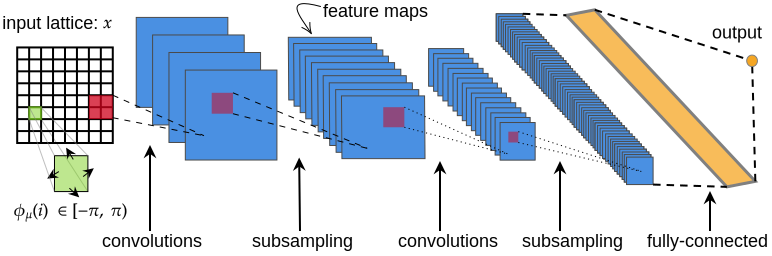
\includegraphics[width=\textwidth]{conv_net/conv_net.pdf}
  % 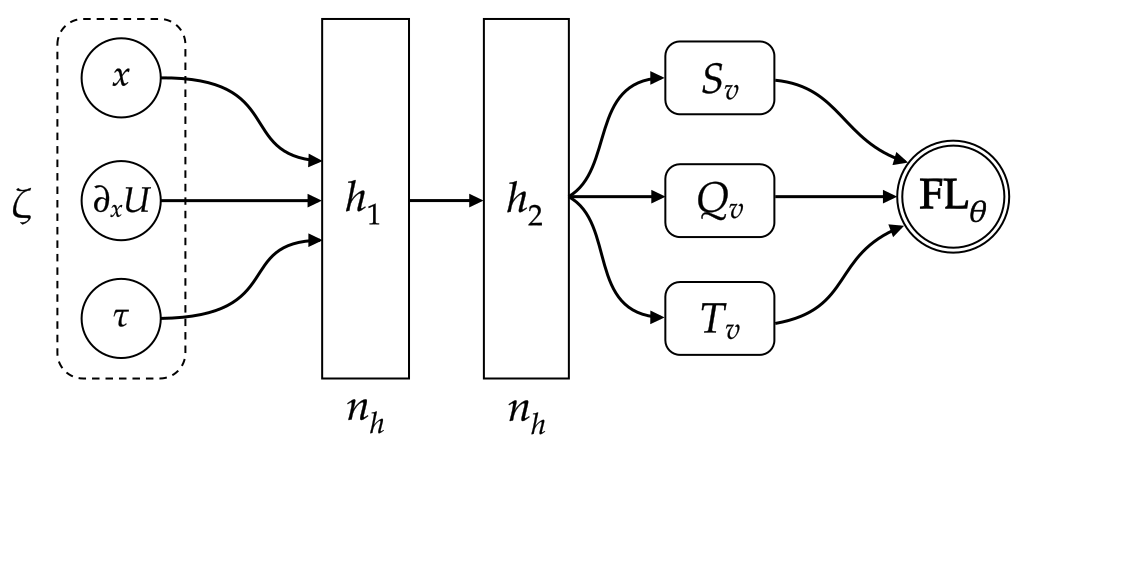
\includegraphics[width=\textwidth]{full_network/generic_net.png}
  \caption{Convolutional structure used for learning localized features of
    rectangular lattice.}%
\label{fig:conv_net}
\end{figure}
% \vspace{-40pt}
%
\begin{figure}[htpb]
  \centering
  \includegraphics[width=0.95\textwidth]{conv_net/vnet_hq.png}
  \caption{Illustration taken from TensorBoard showing an overview of the network architecture for VNet. Note that the
    architecture is identical for XNet.}
    \vspace{12pt}
  \includegraphics[width=0.95\textwidth]{conv_net/vnet_zoom_hq.png}
  \caption{Detailed view of additional convolutional structure included to better account for rectangular geometry of
  lattice inputs.}
\end{figure}
%
Additionally, the network architecture was modified to include a batch normalization layer after the second MaxPool
layer.
%
Introducing batch normalization is a commonly used technique in practice, and is known to help prevent against
diverging gradients\footnote{a numerical issue in which infinite values are generated when calculating the gradients in
backpropagation}, (an issue that was occasionally encountered during the training procedure).
%
Additionally, it has been shown to improve model performance and generally requires fewer training steps to achieve
similar performance as models trained without it~\cite{batch_norm}.
%
\subsection{Annealing Schedule}%
\label{subsec:l2hmc_u1annealing}
% In addition to modifying the neural network architecture, we also modified the training algorithm to follow a simulated
% annealing schedule.
%
Proceeding as in the example of the Gaussian Mixture Model, we include a simulated annealing
schedule in which the value of the gauge coupling $\beta$ is continuously updated according to the annealing schedule
shown in Eq.~\ref{eq:annealing_schedule}.
%
% Explicitly, the value of the gauge coupling $\beta$ is continuously updated according to the annealing schedule shown
% in Eq.~\ref{eq:annealing_schedule}.
%
This was done in order to encourage sampling from multiple different topological charge sectors, since our sampler is
less `restricted' at lower values of $\beta$.
%This was don
\begin{equation}
  \frac{1}{\beta(n)} = {\left(\frac{1}{\beta_{i}} - \frac{1}{\beta_{f}}\right)} {\left(\frac{1 -
  n}{N_{\mathrm{train}}}\right)} + \frac{1}{\beta_{f}}
    \label{eq:annealing_schedule}
\end{equation}
%
Here $\beta(n)$ denotes the value of $\beta$ to be used for the $n^{\mathrm{th}}$ training step ($n = 1, \ldots,
N_{\mathrm{train}}$), $\beta_{i}$ represents the initial value of $\beta$ at the beginning of the training, and
$\beta_{f}$ represents the final value of $\beta$ at the end of training.
%
For a typical training session, $N_{\mathrm{train}} = 25,000$, $\beta_{i} = 2$ and $\beta_{f} = 5$.
% For all of the exmaples above, $N_{\mathrm{train}} = 25,000$, $\beta_{0} = 2$
% and $\beta_{N_{\mathrm{train}}} = 5$.
%
% As can be seen in Fig.~\ref{fig:top_charge}

% \section{UPDATES (04/08/2019)}
%
\subsection{Modified loss function for \texorpdfstring{$U(1)$}{U (1)} gauge model}
\label{subsec:l2hmc_modifiedloss}
%
In order to more accurately define the ``distance'' between two different lattice configurations, we redefine the
metric in Eq.~\ref{eq:metric_orig} to be
%
\begin{equation}
  % \delta(\xi(\phi_{\mu}(x)), \xip(\phi_{\mu}(x))) \equiv 1 - \cos\left(\xi(\phi_{\mu}(x)) - \xi^{\prime}(\phi_{\mu}(x))\right)
  \delta(\xi, \xip) \equiv 1 - \cos\left(\xi - \xi^{\prime}\right)
  \label{eq:metric_new}
\end{equation}
%
where now $\xi \equiv {\left(\phi_{\mu}^{x}(i), \,\phi_{\mu}^{v}(i),\, d\right)}$, with $\phi_{\mu}^{x}$ representing
the lattice of (`position') gauge variables (what we called $x$ previously), and $\phi_{\mu}^{v}$ representing the
lattice of (`momentum') gauge variables (what we called $v$ previously). Note that $i$ runs over all lattice
sites\footnote{In what follows, we will refrain from explicitly including the site index and make the assumption that
it implicitly extends over all sites on the lattice.} and  $\mu=0, 1$ for the two dimensional case.
%
We see that this metric gives the expected behavior, since $\delta \rightarrow 0$ for $\xi \approx \xip$.

While this new metric helps to better measure distances in this configuration space, it does nothing to encourage the
exploration of different topological sectors since there may be configurations for which $\delta(\xi, \xip) \approx 1$
but $Q(\xi) = Q(\xip)$.
%
In order to potentially address this issue, we modify the original loss function as follows.


First define $\xip\equiv \FLq \xi$ as the resultant configuration proposed by the augmented leapfrog integrator, and
%
\begin{align}
  \delta_{Q}{(\xi, \xi^{\prime})} &= \left|Q{(\xi)} - Q{(\xi^{\prime})}\right| \\
  \ell_{Q}{\left(\xi, \xip, A{(\FLq\xi|\xi)}\right)} &= \delta_{Q}{(\xi,\xip)}
    \times A{(\xip|\xi)}.
\end{align}
%
So we have that $\delta_{Q}$ measures the difference in topological charge between the initial and proposed
configurations, and $\ell_{Q}$ gives the expected topological charge difference.
%
Proceeding as before, we include an additional auxiliary term which is identical in structure to the one above, except
the input is now a configuration of link variables $\phi_{\mu}$ drawn from the initialization distribution $q$, which
for our purposes was chosen to be the standard random normal distribution on $[0, 2\pi)$. %]

We can then write the topological loss term as
%
\begin{equation}
  \mathcal{L}_{Q}(\theta) \equiv
    \mathbb{E}_{p(\xi)}{\left[\ell_{Q}{\left(\xi,
      \FLq \xi, A{(\FLq\xi|\xi)}\right)}\right]}
      + \alpha_{\mathrm{aux}}\, \mathbb{E}_{q(\xi)}{\left[\ell_{Q}{\left(\xi,
      \FLq \xi, A{(\FLq\xi|\xi)}\right)}\right]}
      \label{eq:topological_loss_term1}
\end{equation}
%
If we denote the standard loss (with the modified metric function) defined in Eq.~\ref{eq:loss_L} as
$\mathcal{L}_{\mathrm{std}}{(\theta)}$, we can write the new total loss as a combination of these two terms,
%
\begin{equation}
  \mathcal{L}(\theta) =
    \alpha_{\mathrm{std}}\, \mathcal{L}_{\mathrm{std}}(\theta) 
    + \alpha_{Q}\, \mathcal{L}_{Q}(\theta)
    \label{eq:topological_loss_term}
\end{equation}
%
where $\alpha_{\mathrm{std}}, \alpha_Q$ are multiplicative factors that weigh the relative contributions to the total
loss from the standard and topological loss terms respectively, and $\alpha_{\mathrm{aux}}$ in
Eq.~\ref{eq:topological_loss_term1} weighs the contribution of configurations drawn from the initialization
distribution.
%
\subsection{Issues with the Average Plaquette}
%
Upon further testing, an issue was encountered in which the average plaquette $\langle \phi_{P}\rangle$ seems to
converge to a value which is noticeably different from the expected value in the infinite volume limit.
%
This behavior can be seen in Fig.~\ref{fig:bad_convergence}, and seems to depend on both the number of augmented
leapfrog steps used by our integrator, as well as the `strength' of the topological loss term in
Eq.~\ref{eq:topological_loss_term}.
%
The parameters used in Fig~\ref{fig:bad_convergence} are as follows: $L = 8$, $N_{\mathrm{LF}} = 7$, $\alpha_{Q} =
0.5$, and $N_{\mathrm{samples}} = 128$, $N_{\mathrm{train}} = 1\times10^{4}$.
%
In Fig~\ref{fig:good_convergence}, the only change was the weight factor for the topological charge term in the loss
function $\alpha_{Q} = 0$.
%
\begin{figure}[htpb]%
\label{fig:bad_convergence}
  \centering
  % \begin{subfigure}{\textwidth}%
    \includegraphics[width=0.49\textwidth]{plaq_plots/plaqs_vs_step_bad.pdf}
    \includegraphics[width=0.49\textwidth]{plaq_plots/plaqs_diffs_vs_step_bad.pdf}
    \caption{\textbf{(left)}: Average plaquette $\langle\phi_{P}\rangle$ vs.\ step
      for $L=8$, $N_{\mathrm{LF}} = 7$, and $\alpha_{Q} = 0.5$ \textbf{(right)}: Difference between the observed and
      expected value of the average plaquette $\delta_{\phi_{P}}$ vs.\ step. Note that $\delta_{\phi_{P}} \neq 0$.}
\end{figure}
  % \end{subfigure}
  % \vspace{1em}
\begin{figure}[htpb]%
\label{fig:good_convergence}
  \vspace{-20pt}
  \centering
  % \begin{subfigure}{\textwidth}%
    \includegraphics[width=0.49\textwidth]{plaq_plots/plaqs_vs_step_good.pdf}
    \includegraphics[width=0.49\textwidth]{plaq_plots/plaqs_diffs_vs_step_good.pdf}
    \caption{Same quantities as in Fig~\ref{fig:bad_convergence}, with $\alpha_{Q} = 0$. Note that the discrepancy
      $\delta_{\phi_{P}}$ is no longer present.}
  % \end{subfigure}
\end{figure}
    % Each colored line represents a unique chain, and the black line shows the
    % average over all chains.  (left) $\alpha_{Q} = 1$, illustrating the failure
    % to converge to the expected value (denoted by the solid red line), while
    % (right) $\alpha_{Q} = 0$ behaves as expected.}
% \end{figure}
% %
% \begin{figure}[htpb]\label{fig:good_convergence}
  % \centering
  % \caption{(left) Average plaquette $\langle\phi_{P}\rangle$ vs.\ step for $L=8$; (right) the difference between the
  %   observed and expected value in the infinite volume limit (denoted by the red line). Note that $\langle
  % \phi_{P}\rangle$ converges to the expected value in this case.}
%
In order to quantify this unexpected behavior, we can calculate the difference between the observed value of the
average plaquette, $\langle \phi_{P}\rangle$ and the expected value $\phi_{P}^{(*)}$:
% we denote by $\phi_{P}^{(\mathrm{obs})}$ the \emph{observed} value of
% the average plaquette $\phi_{P}$ and $\phi_{P}^{(\mathrm{exp})}$ the \emph{expected} value, we can define the quantity
% 
\begin{equation}
  {\delta_{\phi_P}}(\alpha_Q, N_{\mathrm{LF}}) \equiv \langle \phi_P\rangle - \phi_{P}^{(*)} \neq 0
  % - \langle{\phi_{P}^{\mathrm{(exact)}}}\rangle \neq 0}.
\end{equation}
%
Which allows us to measure the severity of this discrepancy.%
%
% After many unsuccessful attempts and determining the cause of this behavior, I'm still not entirely sure what is
% causing it.
%
% The difference between the observed value and the expected value also seems to increase as more leapfrog steps are
% performed per MD update as well.

Initially it was believed that this behavior was due to the topological charge term in the loss function, however after
testing using $\alpha_{Q} = 0$, this behavior was still present.
%
Following this initial test, it was discovered that the discrepancy seemed to be more prevalent when using a larger
number of leapfrog steps $N_{\mathrm{LF}}$.
%
In an additional systematic attempt to debug the problem, the sampler was trained and evaluated multiple times over a
range of different values of both $N_{\mathrm{LF}}$ and $\alpha_{Q}$.
%
These results are included in Sec.~\ref{chap:debugging_results}.
%
Frustratingly, the issue seemed to be almost irreproducible.
%
Running the training/evaluation processes multiple times using the exact same set of initial parameters on the exact
same hardware it was observed that sometimes the discrepancy was present while other times it was not.

% Also, as expected, when ran for the same number of leapfrog steps and everything else being the same, the difference
% between the observed and expected value of $\langle\phi_{P}\rangle$ increases as $\alpha_{Q}: 0 \rightarrow 1$.
%
% As Xiao-Yong suggested that it might be due to precision issues or round-off errors being carried through, I tried
% re-running everything using \texttt{float64} instead of \texttt{float32} but it didn't seem to make any difference,
% $\langle\phi_{P}\rangle$ still failed to converge to the expected value.

% As an alternative, I've also tried replicating te $\ell$ term from the original loss function Eq.~\ref{eq:loss_ell}
% exactly with $\delta(\xi,\xip) \rightarrow \delta_{Q}(\xi,\xip)$ but this proved to be very unstable and the network
% was unable to get more than a few training steps in before diverging.

% Additionally, I tried repeating the training/evaluation process using
% multiple different values of both $N_{\mathrm{LF}}$ and $\alpha_Q$ ($\alpha_Q$ defined in
% Eq.~\ref{eq:topological_loss_term}).
%
% Strangely, the issue seems to be almost irreproducible and doesn't seem to follow a clear dependence on either
% $N_{\mathrm{LF}}$ or $\alpha_Q$.
%
% I've included plots illustrating the difference $\delta_{\phi_{P}}$ vs. MD step\footnote{Note that each molecular
% dynamics (MD) step consists of a momentum refreshment followed by $N_{\mathrm{LF}}$ leapfrog steps, and finally a
% Metropolis-Hastings accept/reject.} below obtained using both the trained L2HMC sampler as well as the generic HMC
% sampler for comparison.

\section{Conclusion}%
\label{sec:l2hmc_conclusion}
% ---------------------------------------------------------------------------------------------------------------------
% In particular, by drawing a series of correlated samples from a well-defined proposal, our collection of samples will
% converge in distribution to the target equilibrium distribution $\pi$, a technique known as Markov Chain Monte Carlo
% (MCMC) sampling.
% %
% MCMC methods are asymptotically unbiased and remain applicable even in cases when we are not able to sample from $\pi$
% directly, making them a versatile class of algorithms that are widely used across a variety of scientific disciplines.
% %
% While MCMC methods undoubtedly provide an incredibly useful set of tools for
% ---------------------------------------------------------------------------------------------------------------------
In conclusion, we have seen how the Hamiltonian Monte Carlo algorithm follows from the Metropolis-Hastings algorithm
used in generic Markov Chain Monte Carlo methods, and why this approach is often preferred when attempting to sample
from the high-dimensional distributions characteristic of lattice gauge theory models.

% as well as the possible benefits and downsides of
% MCMC methods are defined and used in practice to
Following this, a detailed description of the Hamiltonian Monte Carlo algorithm was presented, as well as some of the
common issues faced when it is applied to lattice quantum chromodynamics.
%
In order to address some of these issues, we then proceeded to introduce a learned inference architecture that
successfully generalized HMC by augmenting the traditional leapfrog integrator with a set of carefully-chosen functions
which are parameterized by weights in a neural network.
%
This system is then trained to learn a MCMC kernel that encourages fast mixing and convergence to the target
distribution.
%
While this transition kernel is no longer symplectic, we are able to retain the strong theoretical gaurantees of HMC by
enforcing a tractable MH accept/reject step, making L2HMC potentially capable of sampling from very challenging
distributions.
%
Having introduced the necessary background, we then looked at applying this algorithm to the notoriously difficult
two-dimensional Gaussian mixture model.
%
In doing so, we found that the trained L2HMC sampler was capable of successfully mixing between modes in a way that
traditional HMC was not.
%
Additionally, we looked at the autocorrelation spectra of samples generated from the trained L2HMC sampler compared to
those obtained from HMC.
%
It was observed that the L2HMC sampler was able to produce samples which were noticeably less correlated in far
fewer steps, indicating that the L2HMC algorithm significantly outperforms traditional HMC.
%
In lattice QCD simulations, the ability of a sampler to quickly produce uncorrelated samples is one of the most
important metrics for measuring its efficiency, and the approach outlined in this chapter shows promise in reducing
the amount of computational resources required to generate new lattice configurations. 

% and allows us to quantify the improvements achieved by alternative
% sampling methods.

% gained as we seek-out and
% identify new met
% and as we seek-out more efficient sampling methods, this allow
%
%
% an important metric
% compared this to the autocorrelations of samples obtained from traditional HMC.
% %
% I
%
%
% , where it was found that the L2HMC algorithm significantly outperformed generic
% HMC.
% %
%
% sampling for the case of the two-dimensional Gaussian Mixture Model,\@ as demonstrated by the trained samplers
% ability to tunnel between
% modes successfully, as well as the drastic improvement in the autocorrelation spectrum.
% %
% All in all, the approach outlined in this chapter shows promise in improving the efficiency of HMC samplers,
% particularly within the context of lattice gauge theory and lattice QCD.
%
It remains to be seen how this algorithm performs when applied to more complicated models (e.g.\ models with fermions
and non-abelian gauge theories), a direction I plan to investigate more carefully in future research.
%
The other, seemingly non-fundamental issue with this approach is the discrepancy between the observed and expected
value of the average plaquette.
%
As of now, I am inclined to believe that this is more of a `bug' than an inherent problem with the algorithm itself.

%
% In this chapter, we have motivated the successfully introduced  the presented a learned inference architecture that
% generalizes HMC by augmenting the traditional leapfrog integrator with a set of carefully-chosen functions which are
% parameterized by weights in a neural network.
%
% This system is then trained to maximize the (suitably chosen) `distance' between successive samples, leading to
%
%
% All things considered, being able to efficiently sample from high-dimensional distributions remains at the heart of
% every MCMC simulation.

MCMC methods have proven to be indispensable in exploring new physics beyond what can be achieved analytically, and has
significantly advanced our understanding of quantum field theory and quantum chromodynamics.
%
% allowing for an independent
% allowing us to gain insight about mechanisms that would otherwise
% us insight into the mechanisms driving the behavior of the world around us.
%
Unfortunately, in order to both perform and  extract meaningful results from these simulations, tremendous amounts of
computational resources are required, with cutting-edge simulations being carried out almost exclusively on some of the
worlds largest supercomputers.

% often calling upon the worlds largest supercomputers.
%
% calling upon the worlds largest supercomputers to be carried out.
%
Because of this, even minor improvements in efficiency can dramatically reduce the amount of computational power
required, allowing for increasingly complex models to be studied.
%
The pursuit of better, more efficient algorithms is one of the major long-term goals of the lattice community, and is
directly aligned with many of the goals outlined for high energy physics in the era of exascale computing. 
%
In particular, the results of these simulations are of central importance to the experiments being carried out at the
Relativistic Heavy Ion Collider at Brookhaven National Laboratory (BNL), and the Large Hadron Collider (LHC) at CERN.

% due to the exponential increase in computational resources resulting from the \emph{critical slowing down} as we
% approach the continuum limit through finer and finer lattice spacings.
%



% and the pursuit of better, more efficient algorithms has led to the discovery of new ways of
% thinking about
% of the
% Being able to sample efficiently from high-dimensional distributions remains one of the primary goals
% simulation.
%
% However, for most distributions of interest, exact posterior inference remains intractable and as a result, approximate
% statistical inference models become necessary.
%

% One family of such algorithms, Markov Chain Monte Carlo (MCMC), allows us to d
% One of the most well-known examples of this type of algorithm is
% Arguably the most well-known and widely used of which being Markov chain Monte Carlo (MCMC) algorithms


% lattice gauge theory and lattice QCD, but

% of gauge generation in
% lattice gauge theory and lattice QCD.
%
%
% generalized the Hamiltonian Monte Carlo algorithm by augmenting the traditional
% leapfrog integrator with a set of carefully-chosen functions which are parameterized by weights in a neural network.
%
% These parameters are trained to encourage fast mixing and convergence to the desired target distribution.
%
%

%%%%%%%%%%%%%%%%%%%%%%%%%%%%%%%%%%%%%%%%%%%%%%%%%%%%%%%%%%%%%%%%%%%%%%%%%%%%%%%%%%%%%%%%%%%%%%%%%%%%%%%%%%%%%%%%%%%%%%%
% \subsection{Systematic Debugging Results}%
% \label{subsec:debugging_results}
% In each of the plots below, the L2HMC sampler was trained for $25,000$ steps with a simulated annealing schedule
% beginning at $\beta = 2.0$ and ending at $\beta = 5.0$.
% %
% Additionally, the training was distributed across $16$ nodes on COOLEY using \texttt{horovod}.
% %
% The results are averaged over all $N_{\mathrm{samples}}$ samples in the
% mini-batch.%
% %
% \begin{figure}[htpb]\label{fig:plaq_diff_plots_lf5}
%   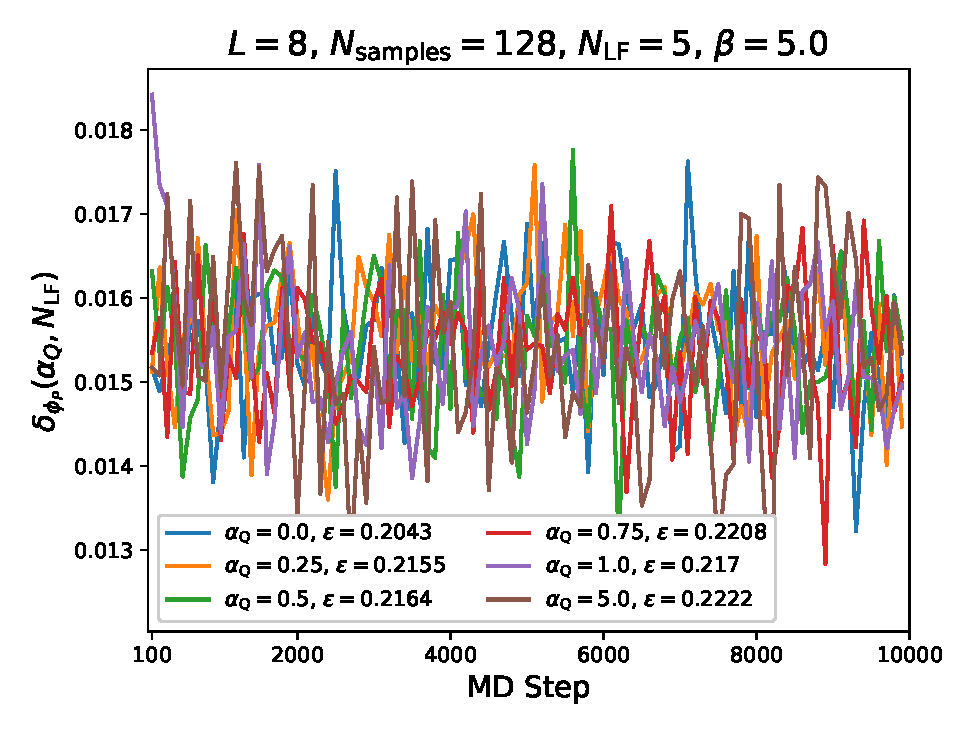
\includegraphics[width=0.49\textwidth]{plaq_difference/plaq_diff_lf5_beta5.eps}
%   \hfill
%   \includegraphics[width=0.49\textwidth]{plaq_difference/plaq_diff_lf5_beta5_HMC.eps}
%   %
%   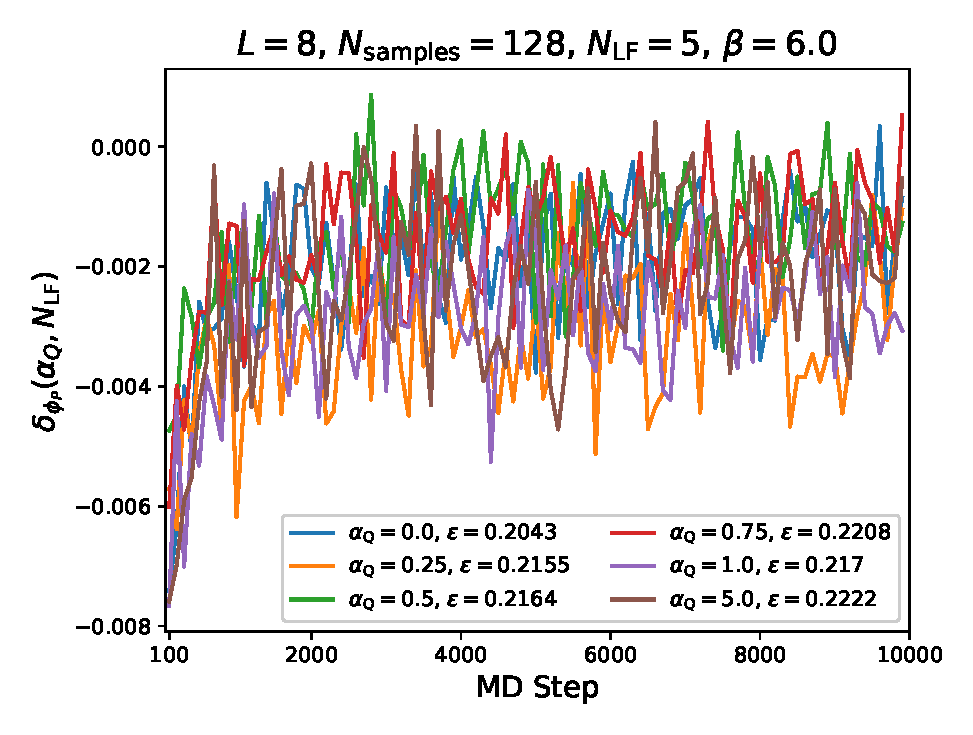
\includegraphics[width=0.49\textwidth]{plaq_difference/plaq_diff_lf5_beta6.eps}
%   \hfill
%   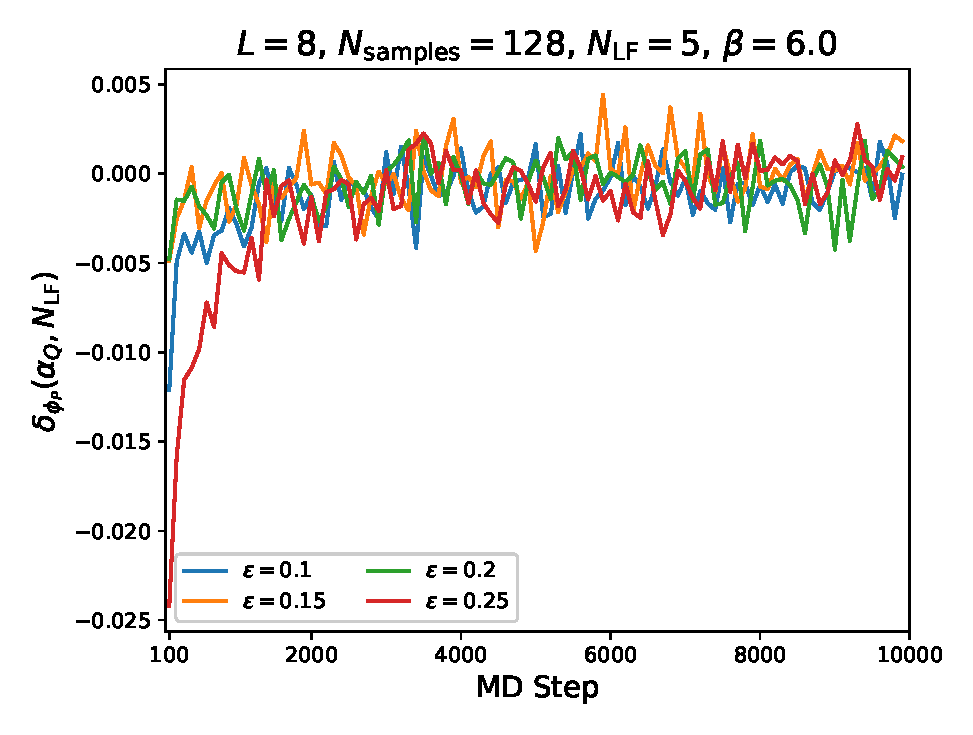
\includegraphics[width=0.49\textwidth]{plaq_difference/plaq_diff_lf5_beta6_HMC.eps}
%   \caption{$\plaqdiff$ vs MD step with $N_{\mathrm{LF}} = 5$ for $\beta = 5.0$ (top row) and $\beta = 6.0$ (bottom
%     row). The results from the trained L2HMC (generic HMC) sampler are shown in the left (right) column. As can be seen,
%     the difference $\delta_{\phi_{P}}$ remains roughly consistent for all values of $\alpha_Q$.}
% \end{figure}
% %
% \begin{figure}[htpb]\label{fig:plaq_diff_plots_lf6}
%   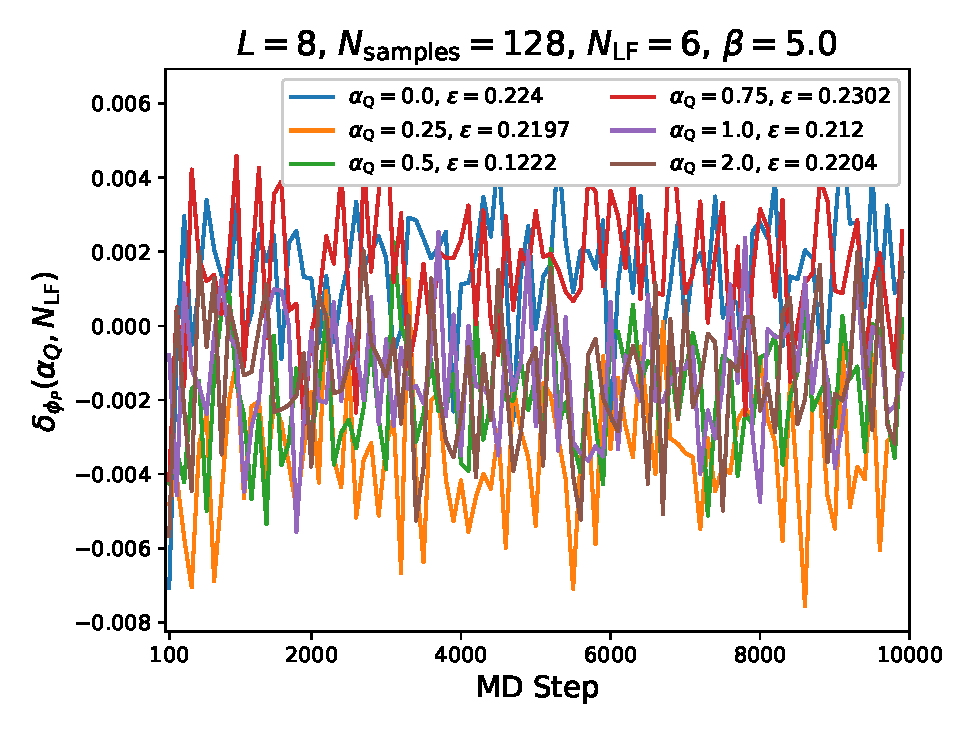
\includegraphics[width=0.49\textwidth]{plaq_difference/plaq_diff_lf6_beta5.eps}
%   \hfill
%   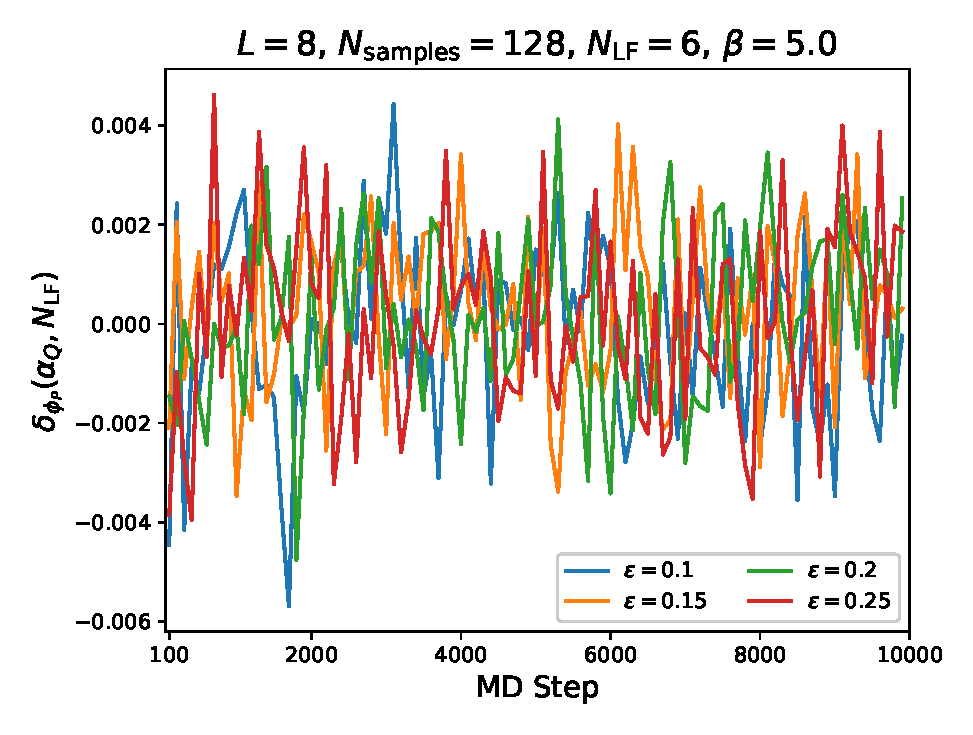
\includegraphics[width=0.49\textwidth]{plaq_difference/plaq_diff_lf6_beta5_HMC.eps}
%   %
%   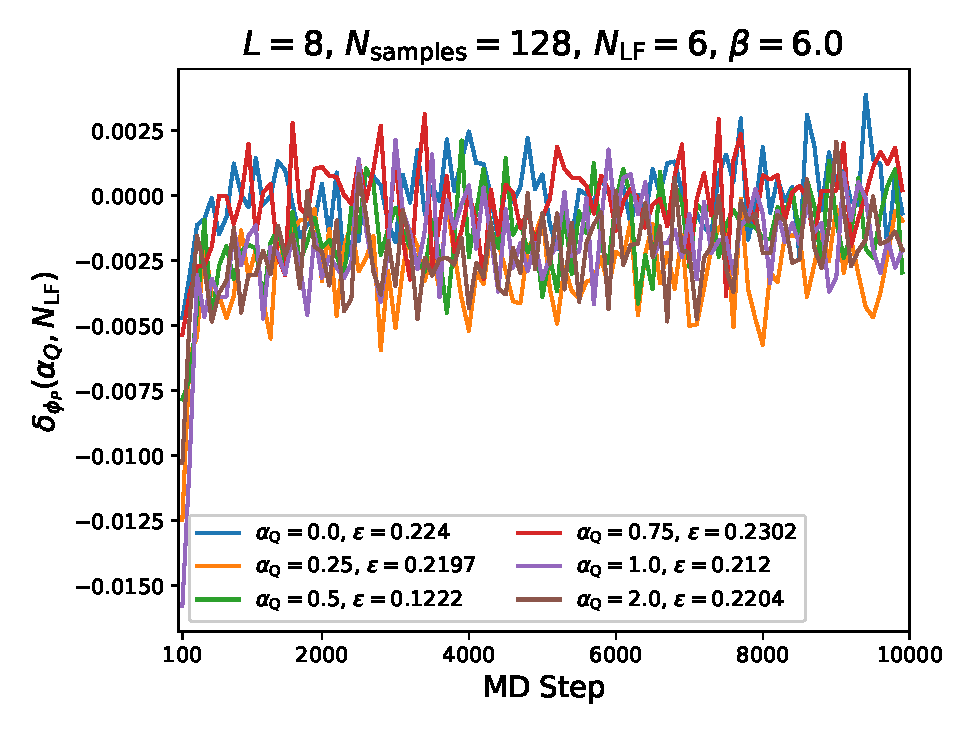
\includegraphics[width=0.49\textwidth]{plaq_difference/plaq_diff_lf6_beta6.eps}
%   \hfill
%   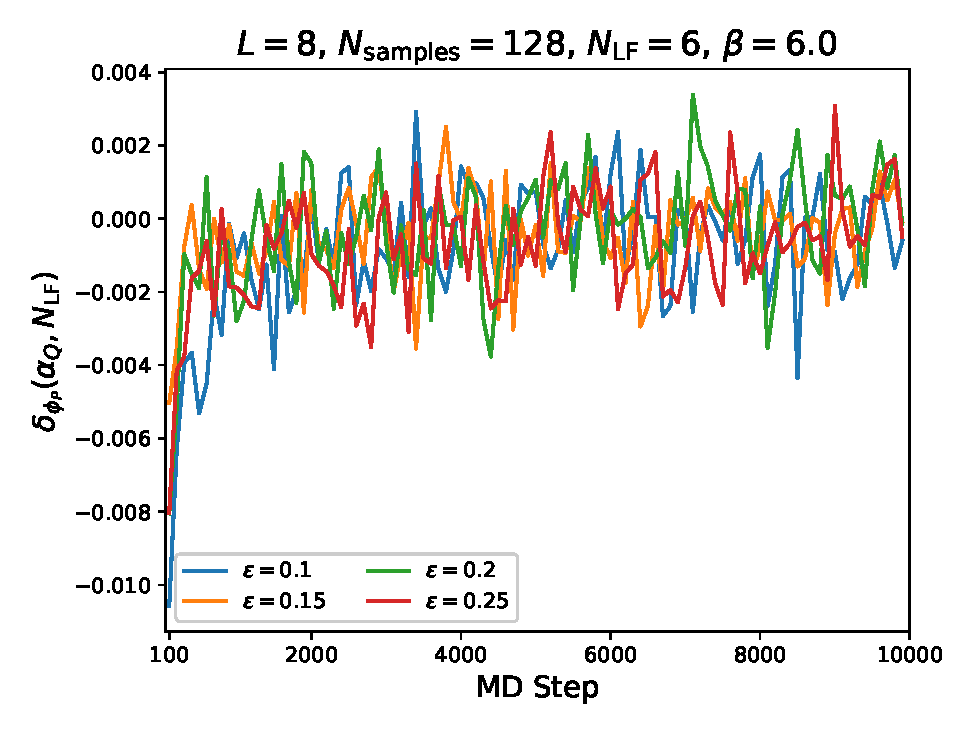
\includegraphics[width=0.49\textwidth]{plaq_difference/plaq_diff_lf6_beta6_HMC.eps}
%   \caption{$\plaqdiff$ vs MD step with $N_{\mathrm{LF}} = 5$ for $\beta = 5.0$ (top row) and $\beta = 6.0$ (bottom
%     row). The results from the trained L2HMC (generic HMC) sampler are shown in the left (right) column. As can be seen,
%     the difference $\delta_{\phi_{P}}$ remains roughly consistent for all values of $\alpha_Q$.}
% \end{figure}
% %
% \begin{figure}[htpb]\label{fig:plaq_diff_plots_lf7}
%   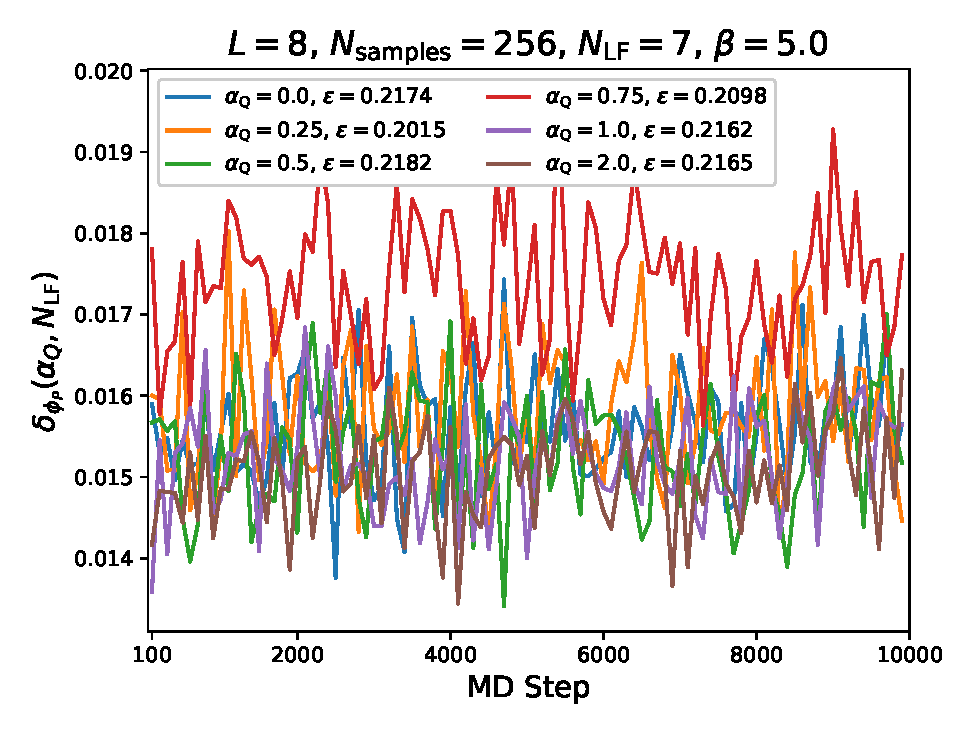
\includegraphics[width=0.49\textwidth]{plaq_difference/plaq_diff_lf7_beta5.eps}
%   \hfill
%   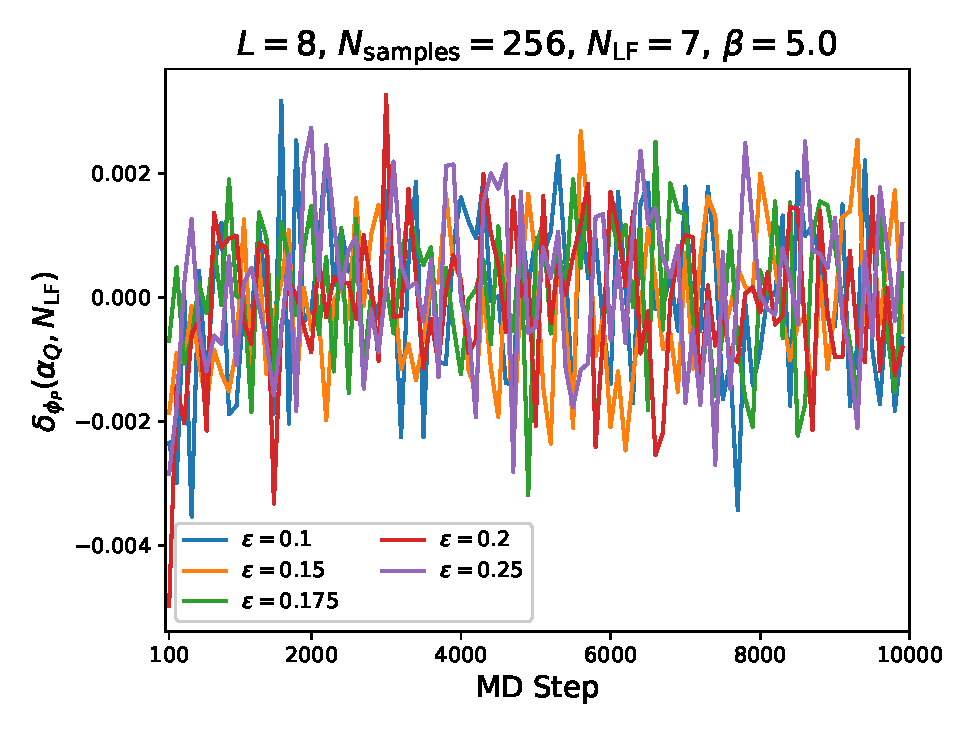
\includegraphics[width=0.49\textwidth]{plaq_difference/plaq_diff_lf7_beta5_HMC.eps}
%   %
%   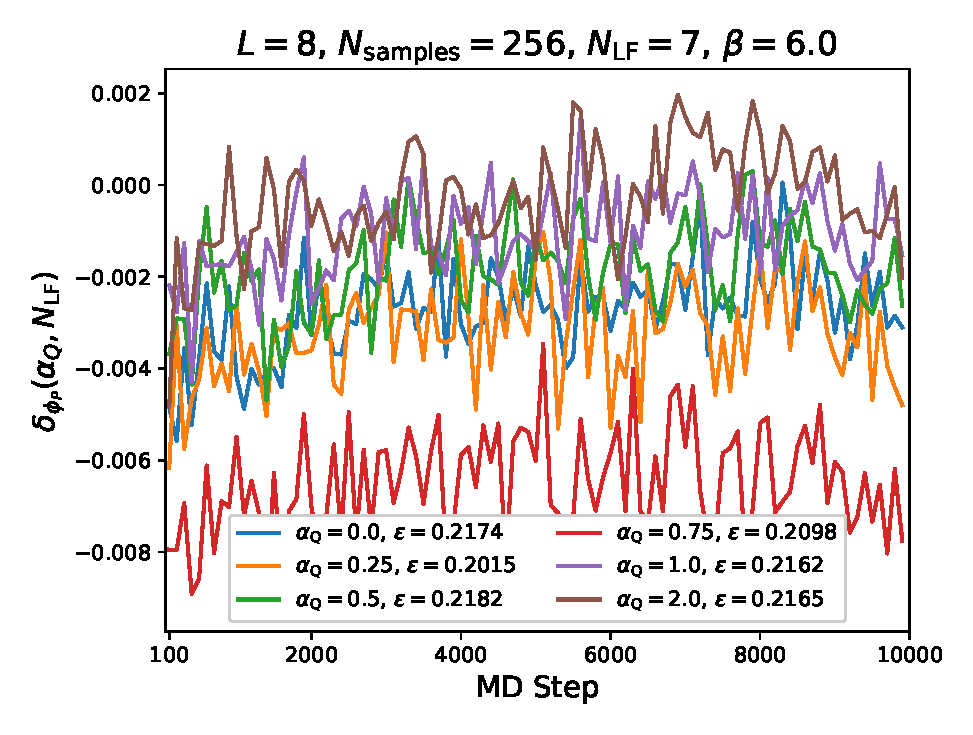
\includegraphics[width=0.49\textwidth]{plaq_difference/plaq_diff_lf7_beta6.eps}
%   \hfill
%   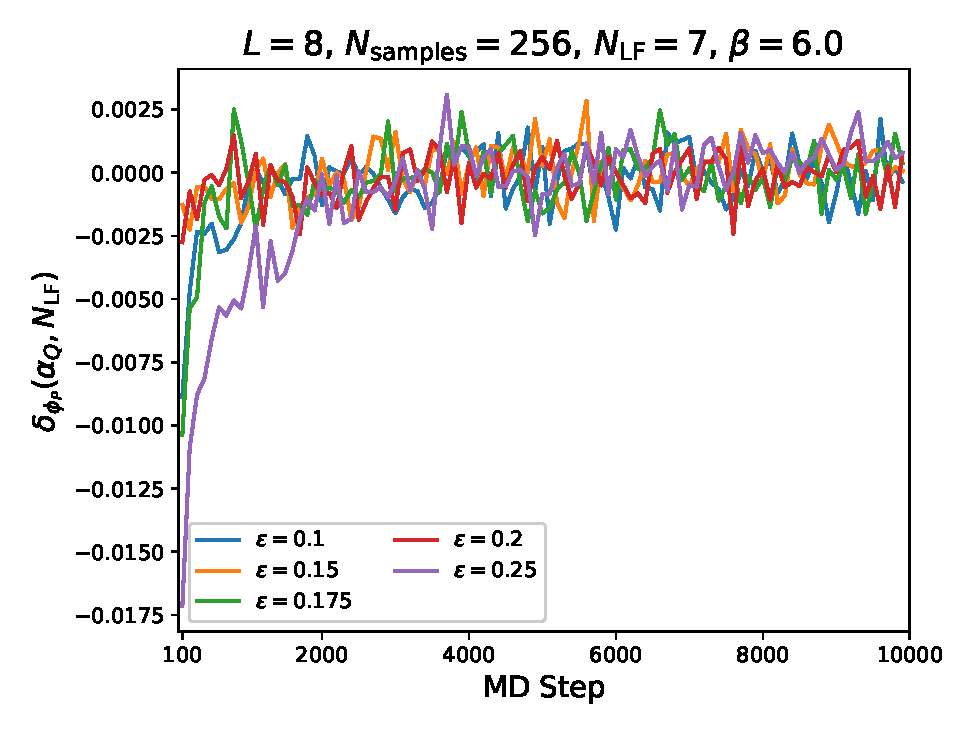
\includegraphics[width=0.49\textwidth]{plaq_difference/plaq_diff_lf7_beta6_HMC.eps}
%   \caption{$\plaqdiff$ vs MD step with $N_{\mathrm{LF}} = 7$ As can be seen, the difference $\delta_{\phi_{P}}$ is
%     noticeably larger for $\alpha_Q = 0.75$, but remains roughly consistent for all other values of $\alpha_Q$.}
% \end{figure}
% %
% \begin{figure}[htpb]\label{fig:plaq_diff_plots_lf8_beta5}
%   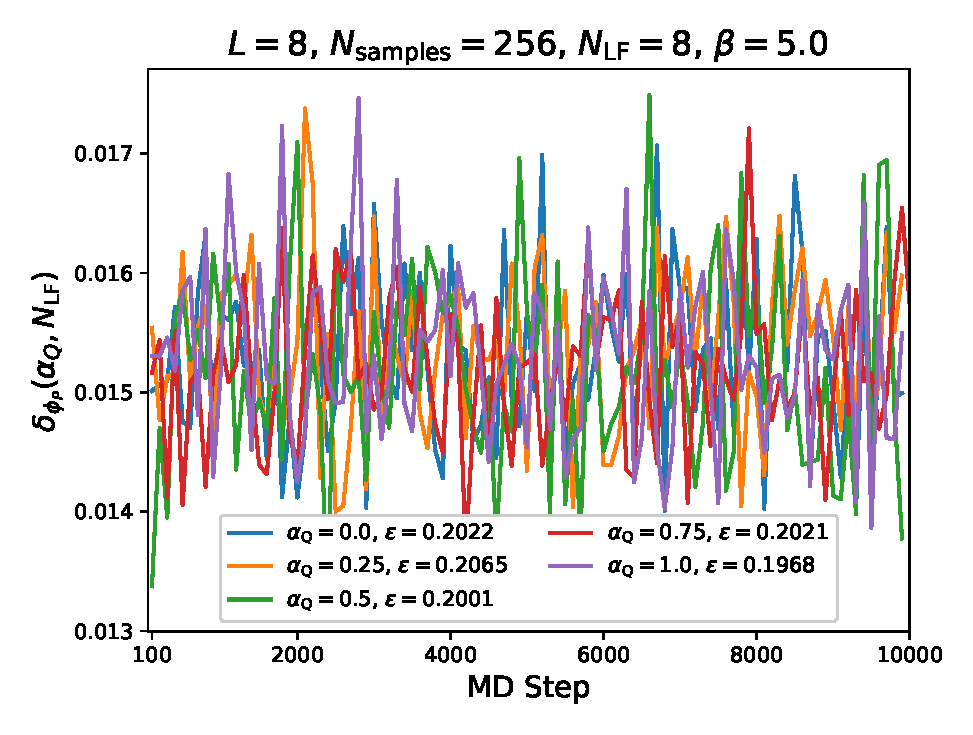
\includegraphics[width=0.49\textwidth]{plaq_difference/plaq_diff_lf8_beta5.eps}
%   \hfill
%   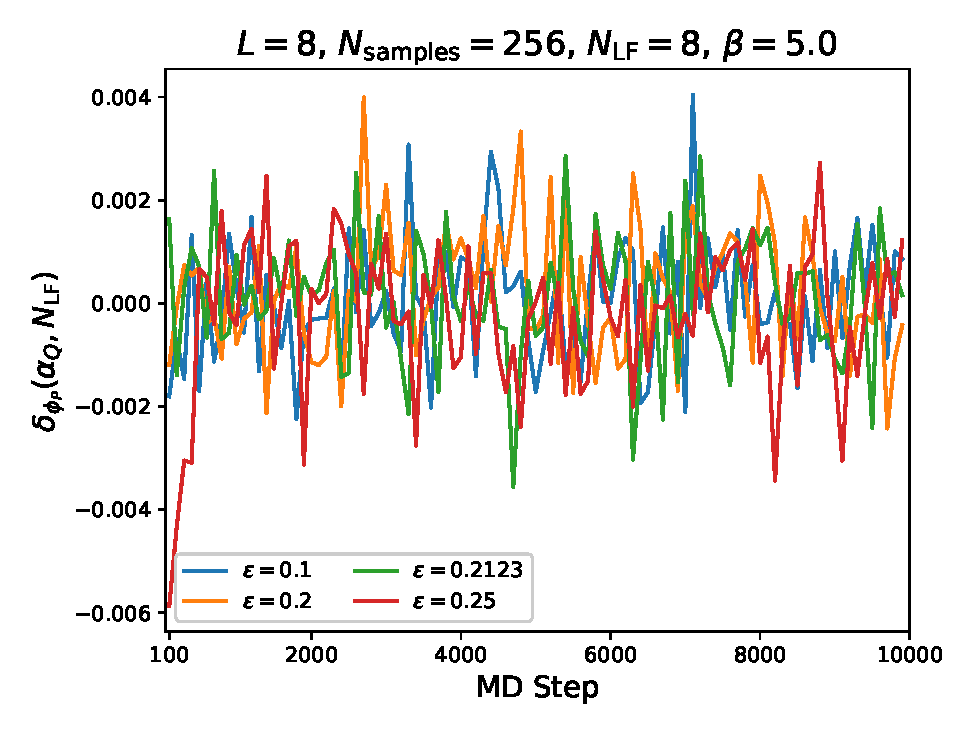
\includegraphics[width=0.49\textwidth]{plaq_difference/plaq_diff_lf8_beta5_HMC.eps}
%   %
%   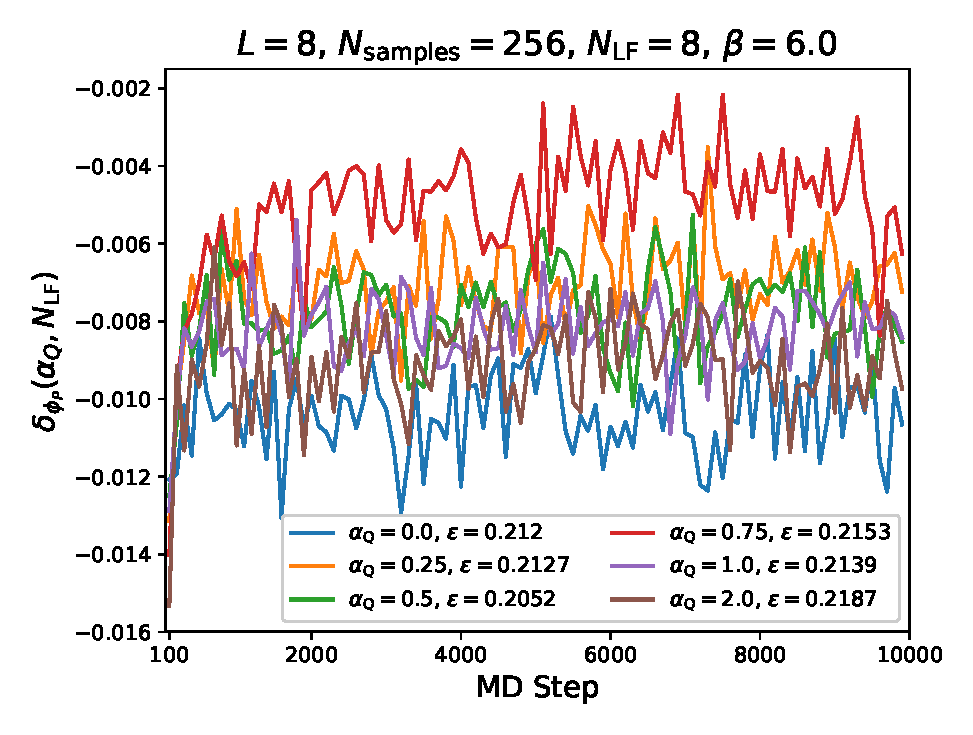
\includegraphics[width=0.49\textwidth]{plaq_difference/plaq_diff_lf8_beta6.eps}
%   \hfill
%   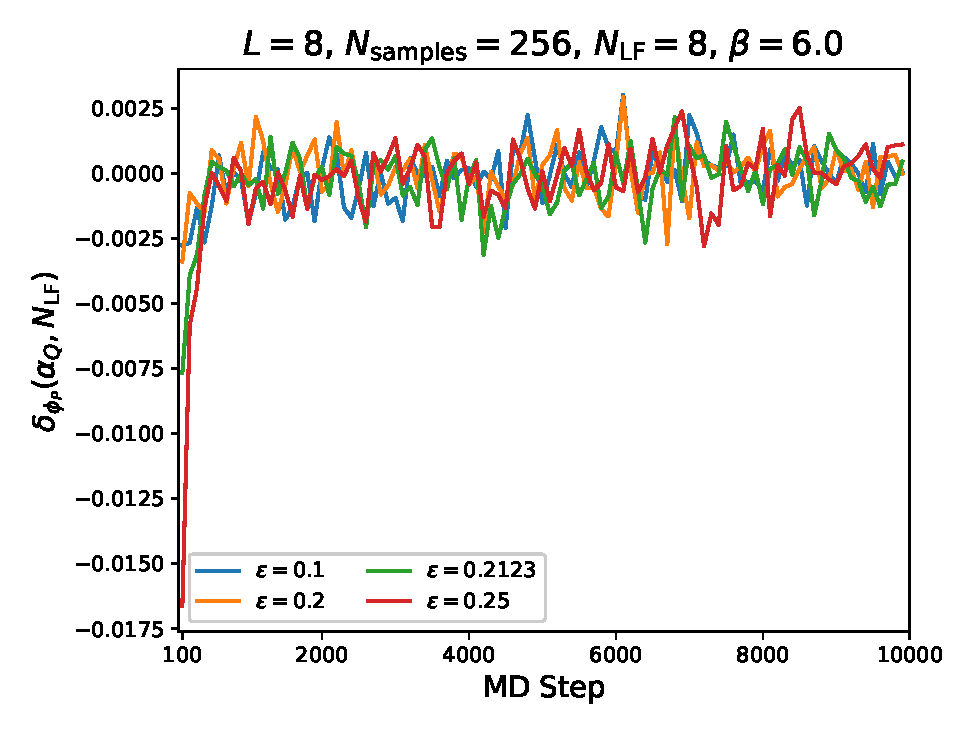
\includegraphics[width=0.49\textwidth]{plaq_difference/plaq_diff_lf8_beta6_HMC.eps}
%   \caption{$\plaqdiff$ vs. MD step with $N_{\mathrm{LF}} = 8$. As can be seen, the difference $\delta_{\phi_{P}}$
%     remains roughly consistent for all values of $\alpha_Q$.}
% \end{figure}
% %
% \begin{figure}[htpb]\label{fig:plaq_diff_plots_lf9}
%   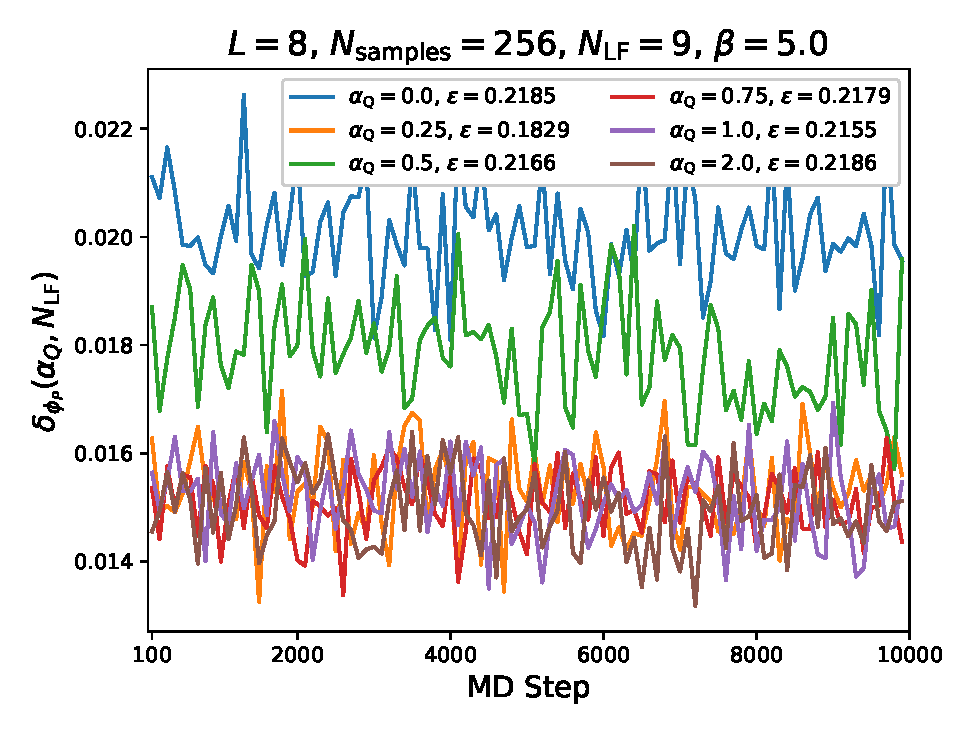
\includegraphics[width=0.49\textwidth]{plaq_difference/plaq_diff_lf9_beta5.eps}
%   \hfill
%   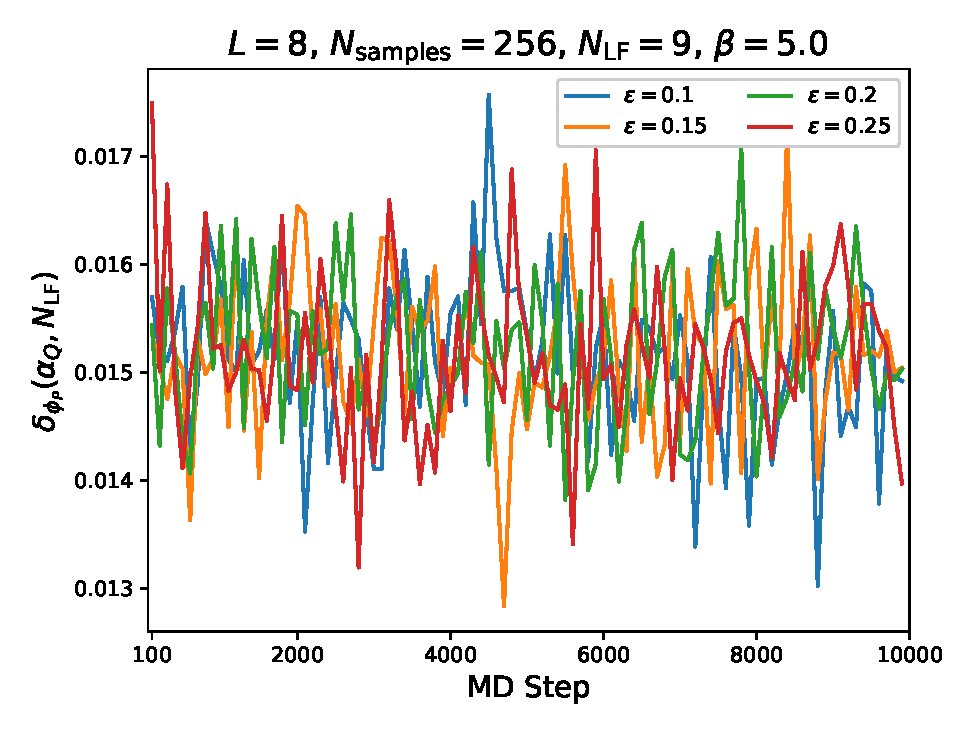
\includegraphics[width=0.49\textwidth]{plaq_difference/plaq_diff_lf9_beta5_HMC.eps}
%   %
%   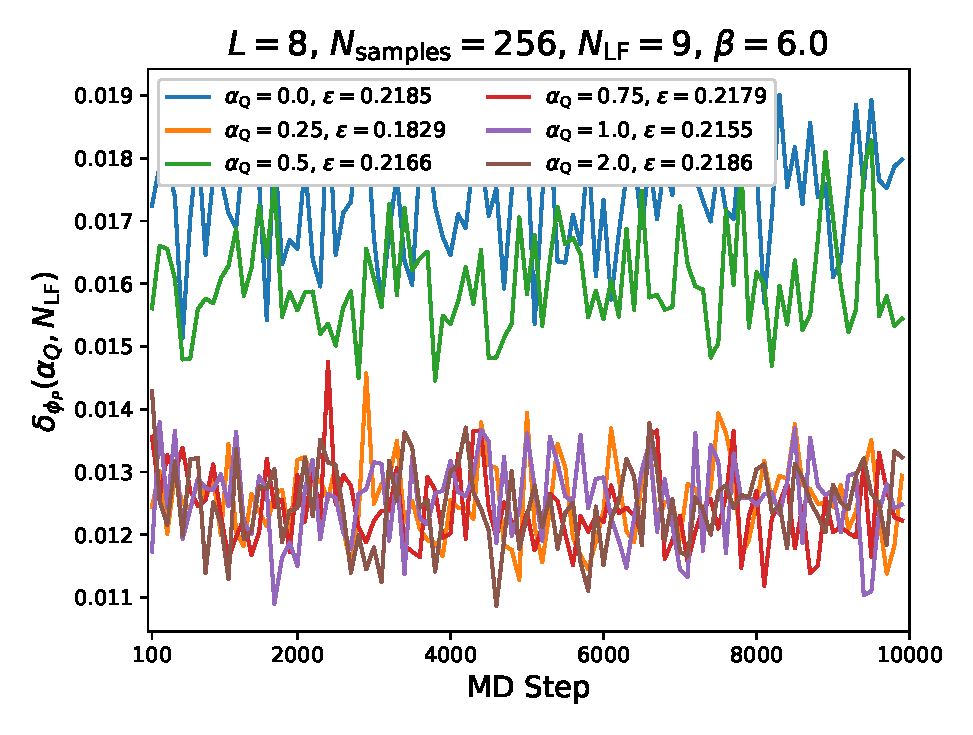
\includegraphics[width=0.49\textwidth]{plaq_difference/plaq_diff_lf9_beta6.eps}
%   \hfill
%   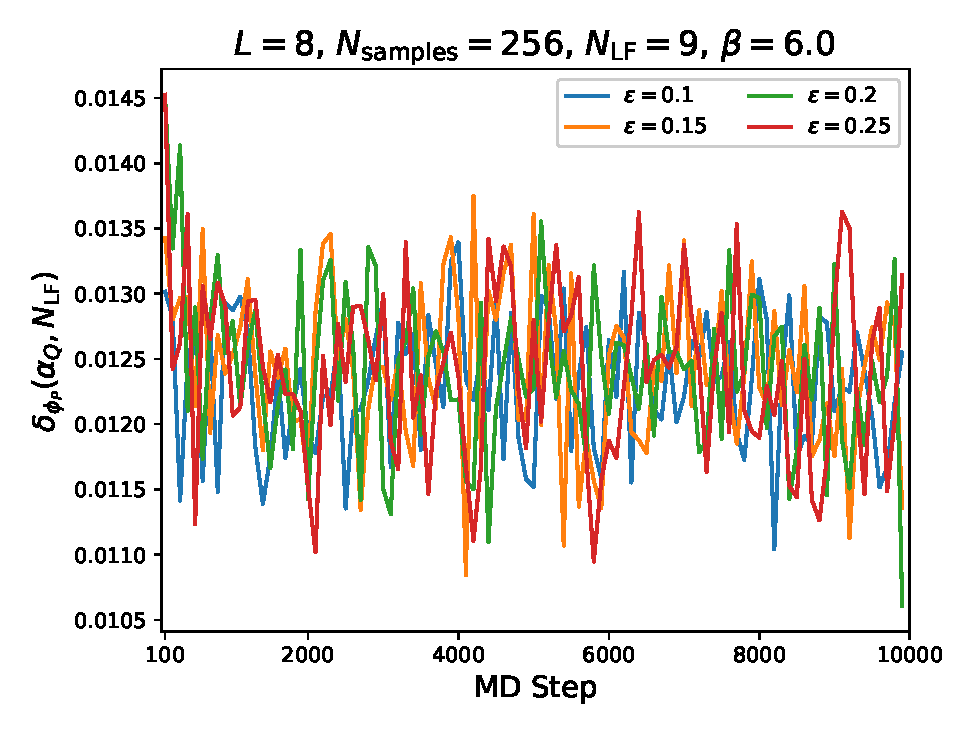
\includegraphics[width=0.49\textwidth]{plaq_difference/plaq_diff_lf9_beta6_HMC.eps}
%   \caption{$\plaqdiff$ vs MD step with $N_{\mathrm{LF}} = 9$. As can be seen, the difference $\delta_{\phi_{P}}$ is
%   largest for $\alpha_Q = 0.0$ and $\alpha_Q = 0.5$.}
% \end{figure}
% %
% \begin{figure}[htpb]\label{fig:plaq_diff_plots_lf10}
%   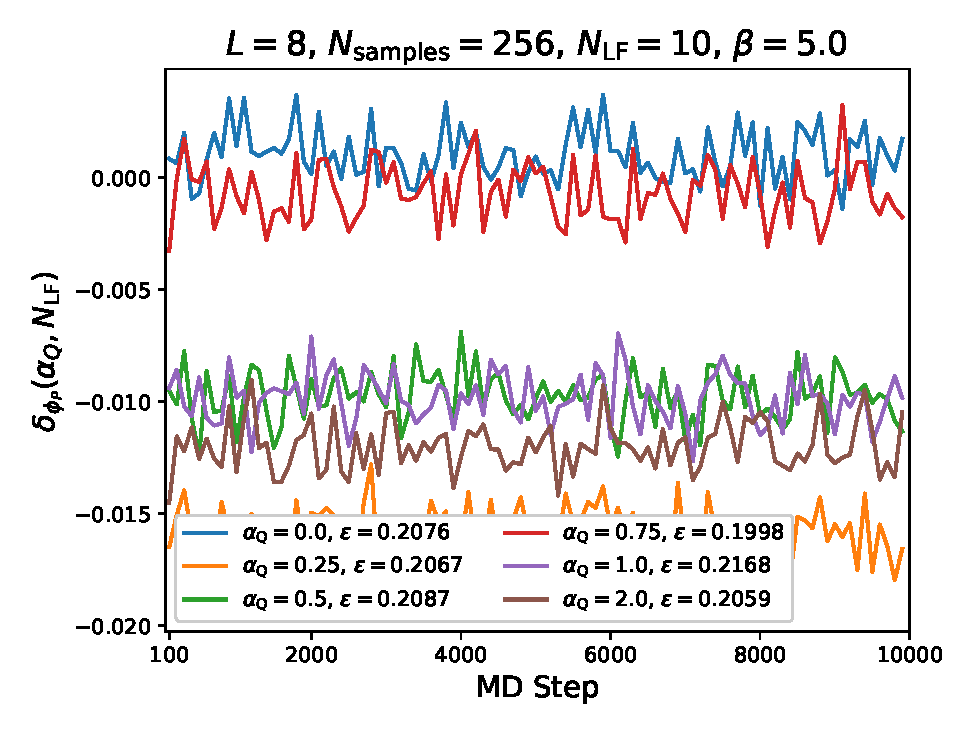
\includegraphics[width=0.49\textwidth]{plaq_difference/plaq_diff_lf10_beta5.eps}
%   \hfill
%   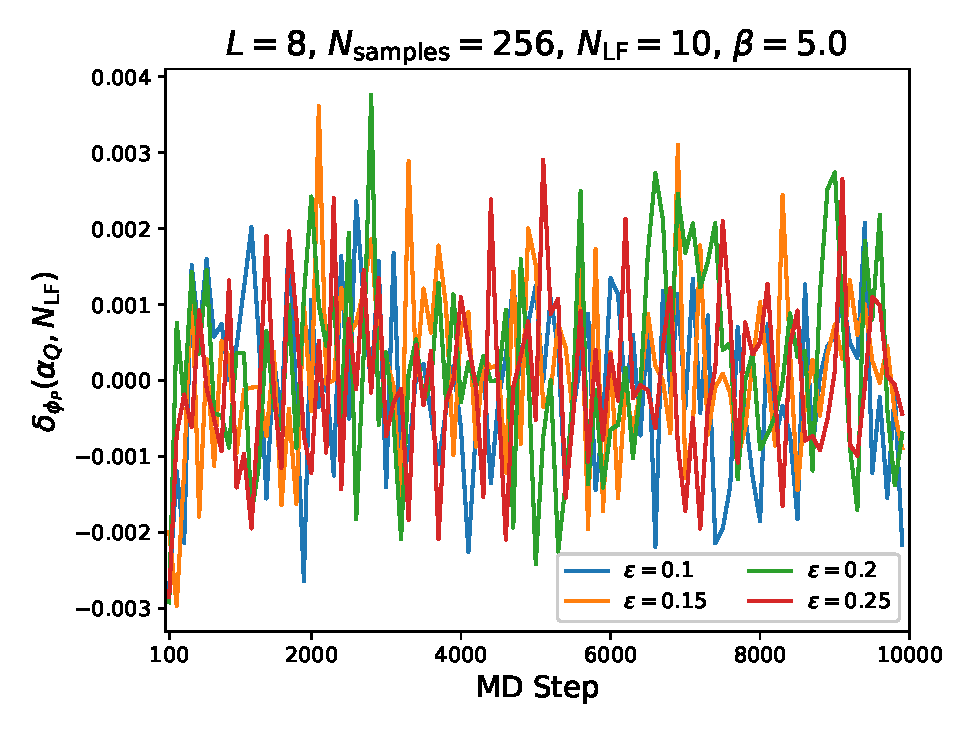
\includegraphics[width=0.49\textwidth]{plaq_difference/plaq_diff_lf10_beta5_HMC.eps}
%   %
%   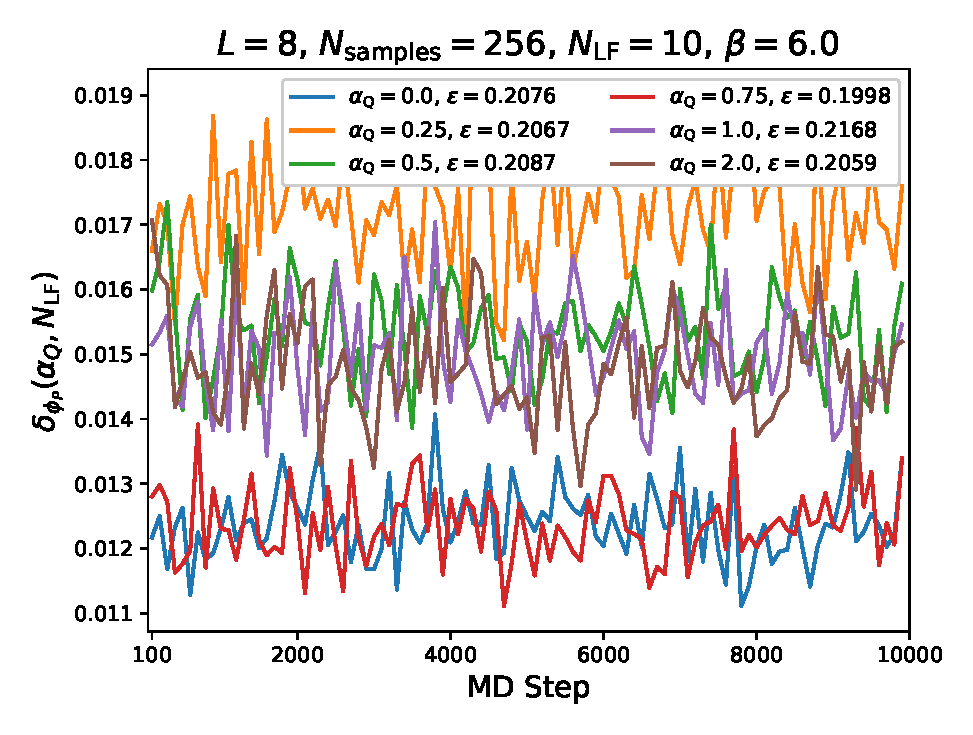
\includegraphics[width=0.49\textwidth]{plaq_difference/plaq_diff_lf10_beta6.eps}
%   \hfill
%   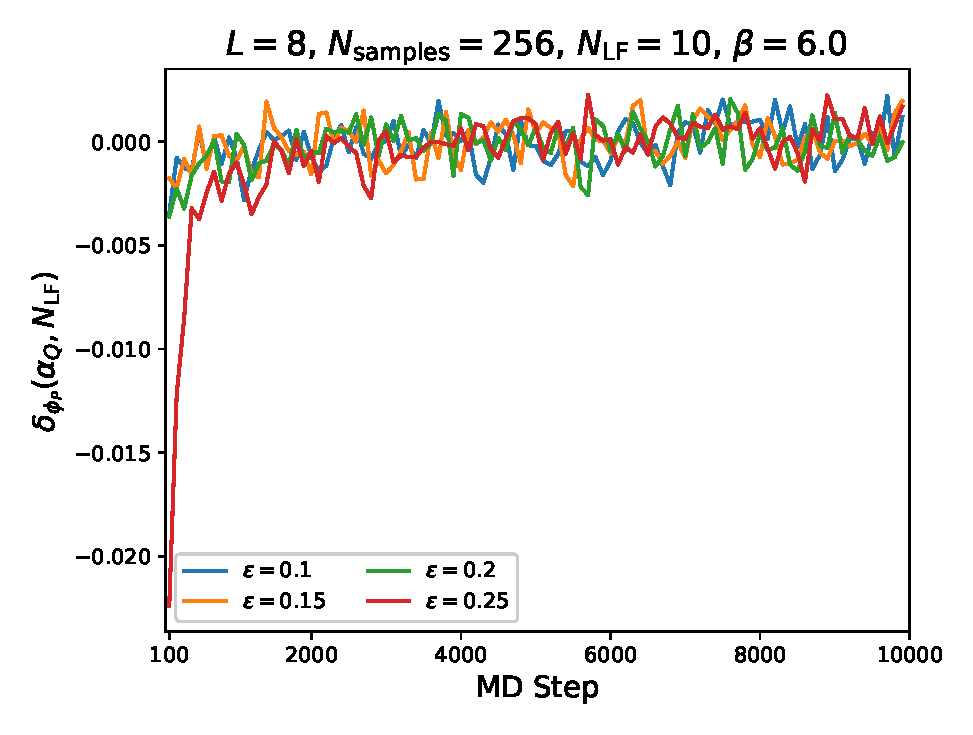
\includegraphics[width=0.49\textwidth]{plaq_difference/plaq_diff_lf10_beta6_HMC.eps}
%   \caption{$\plaqdiff$ vs MD step with $N_{\mathrm{LF}} = 10$. As can be seen, the difference $\delta_{\phi_{P}}$ is
%     smallest for $\alpha_Q = 0.,\,\,0.75$ and largest for $\alpha_Q = 0.25$, while $\alpha_Q = 0.5,\,\,2.0$, takes on
%   intermediate values.}
% \end{figure}
% %
% \begin{figure}[htpb]\label{fig:plaq_diff_plots_lf15}
%   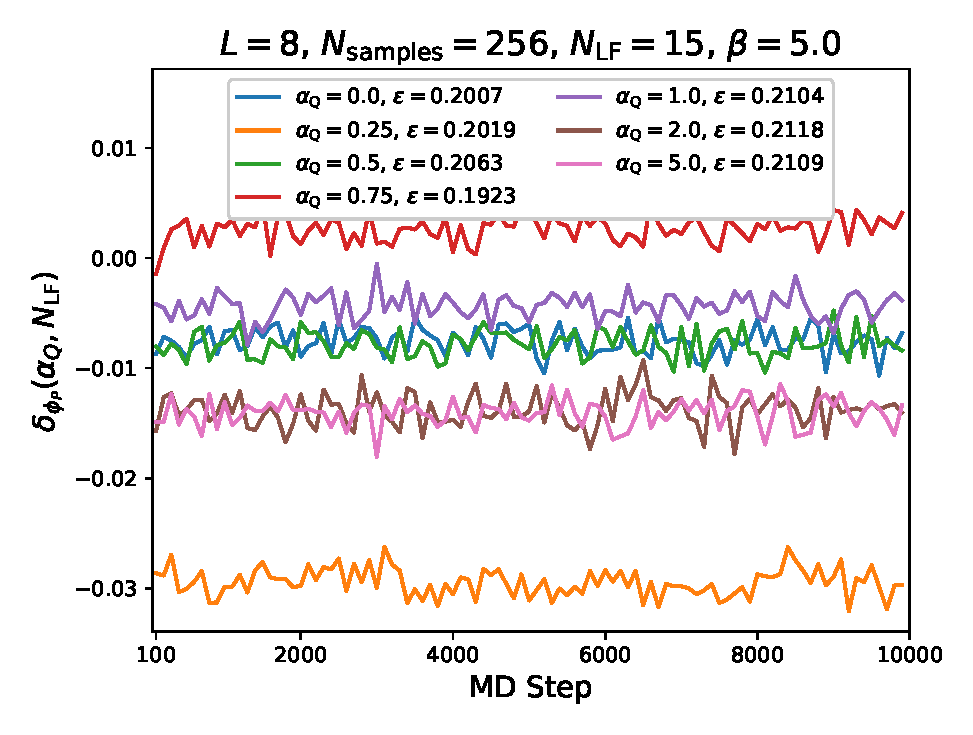
\includegraphics[width=0.49\textwidth]{plaq_difference/plaq_diff_lf15_beta5.eps}
%   \hfill
%   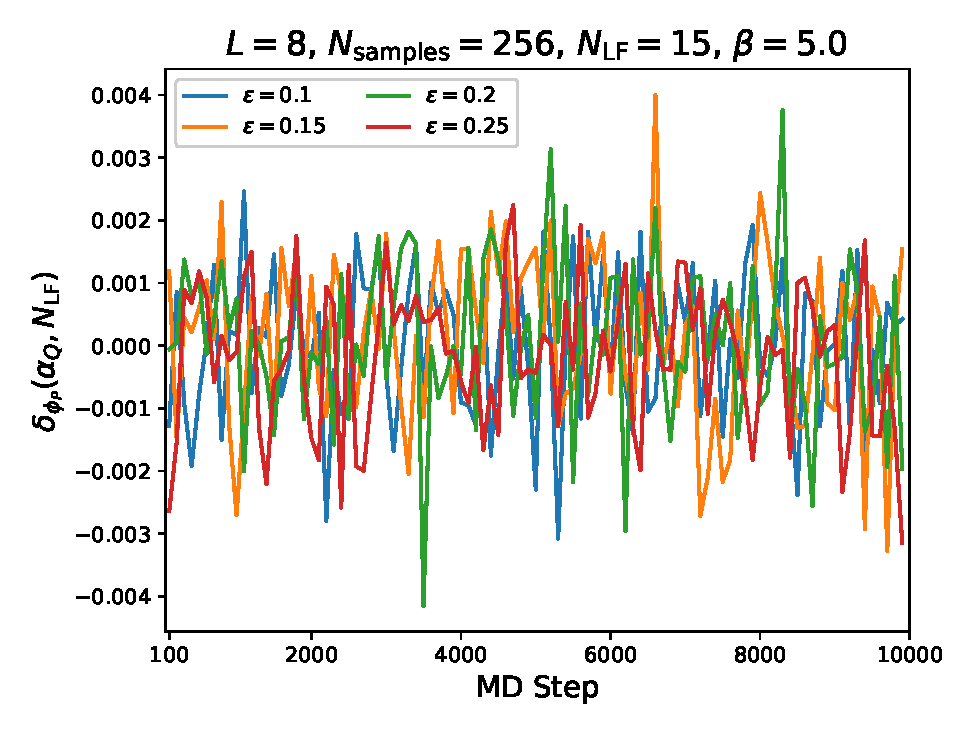
\includegraphics[width=0.49\textwidth]{plaq_difference/plaq_diff_lf15_beta5_HMC.eps}
%   %
%   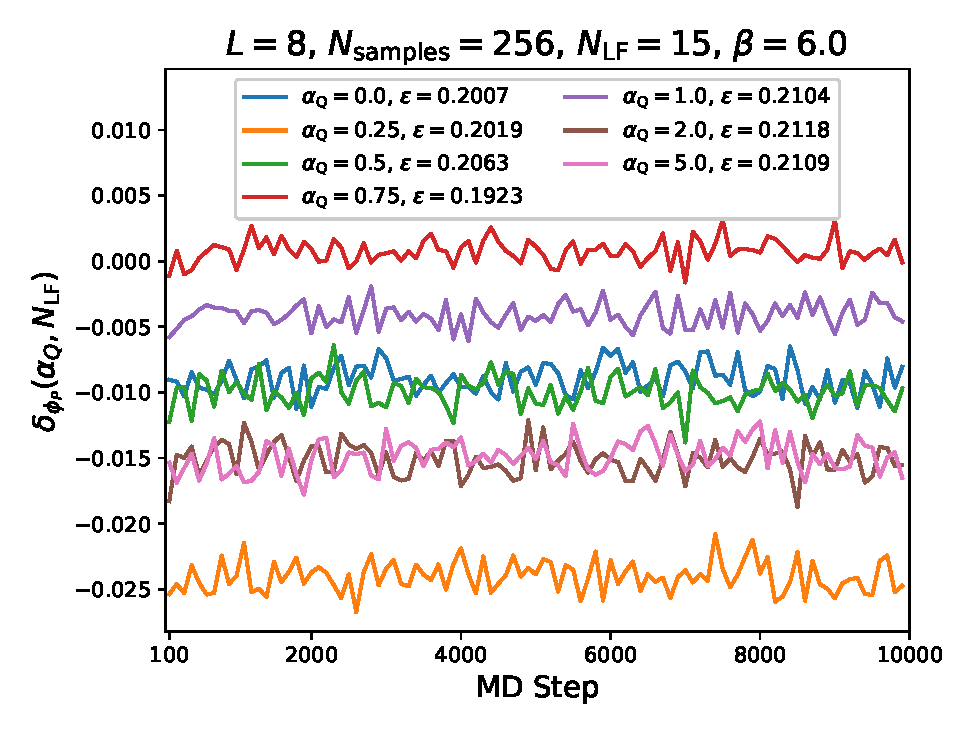
\includegraphics[width=0.49\textwidth]{plaq_difference/plaq_diff_lf15_beta6.eps}
%   \hfill
%   \includegraphics[width=0.49\textwidth]{plaq_difference/plaq_diff_lf15_beta6_HMC.eps}
%   \caption{$\plaqdiff$ vs MD step with $N_{\mathrm{LF}} = 15$. As can be seen, the difference $\delta_{\phi_{P}}$
%     varies for different values of $\alpha_Q$.}
% \end{figure}
%%%%%%%%%%%%%%%%%%%%%%%%%%%%%%%%%%%%%%%%%%%%%%%%%%%%%%%%%%%%%%%%%%%%%%%%%%%%%%%%%%%%%%%%%%%%%%%%%%%%%%%%%%%%%%%%%%%%%%%

% I'm currently working on re-running all of the following experiments to see if this difference $\plaqdiff$ is
% reproducible or if it is some sort of anomaly.

% \subsubsection*{Diverging gradients}
% On a separate `debugging' note, previously I had mentioned that I would occasionally run into an issue where the
% gradients would (seemingly randomly) blow up during training. I had spoken with Xiao-Yong about this in a little more
% depth and I explained that I believed it was directly related to the gradient of the step size, which I was able to
% occasionally avoid by introducing a gradient clipping operation during backpropagation. This approach seemed to work
% well in some cases but would still occasionally diverge.
%
%
% \subsection*{Topological susceptibility \texorpdfstring{$\chi$}{χ:}}
% %
% \begin{figure}[htpb]
%   \centering
%   \includegraphics[width=0.95\textwidth]{suscept_plots/topological_suscept_vs_beta_all_10}
%   \caption{Topological susceptibility vs. $\beta$ for various lattice sizes
%   $L = 8, 12, 16$. Note that the data points in the inset plots are slightly
%   shifted horizontally from each other for illustrative purposes.}%
%   \label{fig:suscept}
% \end{figure}
% %
% \begin{itemize}
%   \item All statistics for $\chi$ were calculated by running either the
%     trained L2HMC sampler or a generic HMC sampler with equivalent
%     parameters (step size at the end of training, number of leapfrog steps,
%     etc.).  %
%   \item For $N_{\mathrm{MD}}$ molecular dynamics (accept/reject) update
%     steps for $N_{\mathrm{chains}}$ (batch size) chains in parallel.  %
%   \item Each molecular dynamics update step consists of $5$ individual
%     leapfrog steps (augmented leapfrog step for L2HMC sampler).  %
%   \item For the results shown in Fig.~\ref{fig:suscept}, $N_{\mathrm{MD}} =
%     1\times10^4$ for all values of $L$, and $N_{\mathrm{chains}} = 32,
%     50, 64$ for $L = 16, 12$, and $8$ respectively.
% \end{itemize}
% %
% \begin{figure}[htpb]%\label{fig:top_charges8_l2hmc}
%   \centering
%   \includegraphics[width=0.49\textwidth]{charge_plots/top_charge_vs_step8_L2HMC}
%   \hfill
%   \includegraphics[width=0.49\textwidth]{charge_plots/top_charge_vs_step8_HMC}
%   \includegraphics[width=0.49\textwidth]{charge_plots/top_charge_vs_step12_L2HMC}
%   \hfill
%   \includegraphics[width=0.49\textwidth]{charge_plots/top_charge_vs_step12_HMC}
%   \includegraphics[width=0.49\textwidth]{charge_plots/top_charge_vs_step16_L2HMC}
%   \hfill
%   \includegraphics[width=0.49\textwidth]{charge_plots/top_charge_vs_step16_HMC}
%   \caption{Topological charge of a single chain vs.\ evaluation step at
%   $\beta=5$. Top row: $L=8$, Middle row: $L=12$, bottom row $L=16$. Left
%   column: trained L2HMC sampler, right column: generic HMC sampler}
% \end{figure}
% %
% \begin{figure}[htpb]%\label{}
%   \centering
%   \includegraphics[width=0.49\textwidth]{charge_plots/top_charge_vs_step8_b4_L2HMC}
%   \hfill
%   \includegraphics[width=0.49\textwidth]{charge_plots/top_charge_vs_step8_b4_HMC}
%   \includegraphics[width=0.49\textwidth]{charge_plots/top_charge_vs_step12_b4_L2HMC}
%   \hfill
%   \includegraphics[width=0.49\textwidth]{charge_plots/top_charge_vs_step12_b4_HMC}
%   \includegraphics[width=0.49\textwidth]{charge_plots/top_charge_vs_step16_b4_L2HMC}
%   \hfill
%   \includegraphics[width=0.49\textwidth]{charge_plots/top_charge_vs_step16_b4_HMC}
%   \caption{Topological charge of a single chain vs.\ evaluation step at
%     $\beta=4$. Top row: $L=8$, Middle row: $L=12$, bottom row $L=16$. Left
%     column: trained L2HMC sampler, right column: generic HMC sampler}
% \end{figure}
%
% \section{UPDATES (04/22/2019) Autocorrelation of topological charge \texorpdfstring{$Q$}{Q}}
% We are interested in the autocorrelation of the topological charge $Q$.
% %
% \begin{figure}[htpb]
%   \centering
%   \includegraphics[width=0.48\textwidth]{autocorrelations/top_charge_autocorrelations_L8_steps3_batch256}
%   \includegraphics[width=0.48\textwidth]{autocorrelations/top_charge_autocorrelations_L8_steps5_batch128}
%   \caption{Autocorrelation of the topological charge $Q$, on an $8 \times 8$
%     lattice, averaged over $128$ samples. The molecular dynamics
%   update consisted of $3$ (left) and $5$ (right) augmented (L2HMC) leapfrog steps.}
%   \label{fig:charge_acorr_L8}
% \end{figure}
% %
% \begin{figure}[htpb]
%   \centering
%   \includegraphics[width=0.48\textwidth]{autocorrelations/top_charge_autocorrelations_L16_steps3_batch256}
%   \includegraphics[width=0.48\textwidth]{autocorrelations/top_charge_autocorrelations_L16_steps5_batch128}
%   \caption{Autocorrelation of the topological charge $Q$, on an $16 \times 16$
%     lattice, averaged over $128$ samples. The molecular dynamics
%   update consisted of $3$ (left) and $5$ (right) leapfrog steps.}
%   \label{fig:charge_acorr_L16}
% \end{figure}
%
% The model was trained using simulated annealing for $N_{\mathrm{train}}$ training steps.
% %
% The paramter $\beta$ was updated according to the annealing schedule shown in Eq.~\ref{eq:annealing_schedule}.
% %
% \begin{equation}
%   \frac{1}{\beta(n)} = {\left(\frac{1}{\beta_{i}} - \frac{1}{\beta_{f}}\right)} {\left(\frac{1 -
%   n}{N_{\mathrm{train}}}\right)} + \frac{1}{\beta_{f}}
%     \label{eq:annealing_schedule}
% \end{equation}
% %
% Here $\beta(n)$ denotes the value of beta to be used for the $n^{\mathrm{th}}$ training step ($n = 1, \ldots,
% N_{\mathrm{train}}$), $\beta_{i}$ represents the initial value of $\beta$ at the beginning of the training, and
% $\beta_{f}$ represents the final value of $\beta$ at the end of training.
% %
% For all of the exmaples above, $N_{\mathrm{train}} = 25,000$, $\beta_{0} = 2$
% and $\beta_{N_{\mathrm{train}}} = 5$.

% \section{UPDATES (05/03/2019)}
% Previously we had noticed that there seems to be a discrepancy between the observed and expected value of the average
% plaquette,
% %
% \begin{equation}
%   {\delta_{\phi_P}(\alpha_Q, N_{\mathrm{LF}}) \equiv \langle \phi_P^{\mathrm{(obs)}}\rangle
%   - \langle{\phi_{P}^{\mathrm{(exp)}}}\rangle \neq 0}.
% \end{equation}
% %
% In an attempt to better understand why this was occurring, I tried repeating the training/evaluation process using
% multiple different values of both $N_{\mathrm{LF}}$ and $\alpha_Q$ ($\alpha_Q$ defined in
% Eq.~\ref{eq:topological_loss_term}).
% %
% Strangely, the issue seems to be almost irreproducible and doesn't seem to follow a clear dependence on either
% $N_{\mathrm{LF}}$ or $\alpha_Q$.
% %
% I've included plots illustrating the difference $\delta_{\phi_{P}}$ vs. MD step\footnote{Note that each molecular
% dynamics (MD) step consists of a momentum refreshment followed by $N_{\mathrm{LF}}$ leapfrog steps, and finally a
% Metropolis-Hastings accept/reject.} below obtained using both the trained L2HMC sampler as well as the generic HMC
% sampler for comparison.
% %
% In each of the plots below, the L2HMC sampler was trained for $25,000$ steps with a simulated annealing schedule
% beginning at $\beta = 2.0$ and ending at $\beta = 5.0$.
% %
% Additionally, the training was distributed across $16$ nodes on COOLEY using \texttt{horovod}.
% %
% The results are averaged over all $N_{\mathrm{samples}}$ samples in the
% mini-batch.
%
% I'm currently working on re-running all of the following experiments to see if this difference $\plaqdiff$ is
% reproducible or if it is some sort of anomaly.
%
%
%
% \include{autocorrelation_plots}
%
% \section{UPDATES (05/15/2019) Debugging convergence issues}
% We mainly want to know:
% \begin{itemize}
%   \item How the plain link variables, $\phi_{\mu}(i) \in [-\pi, \pi)$ change during the leapfrog updates. If we
%     denote by $\phi_{\mu}^{(t)}{(i)}$ an individual link variable at the $t^{th}$ leapfrog step then we can look at how
%     these values change between subsequent leapfrog updates through the quantity
%     \begin{equation}
%       \delta \phi_{\mu}{(i)} = \phi_{\mu}^{(t+1)}{(i)} - \phi_{\mu}^{(t)}{(i)}
%     \end{equation}
%     For illustrative purposes, we can look at how the average link changes and define
%     \begin{align}
%       \langle \delta \phi_{\mu}{(i)}\rangle &= \frac{1}{N_{\mathrm{links}}}\sum_{\mu, i} \delta \phi_{\mu}(i) \\
%     \end{align}
%   %
%   \item How the determinant of the Jacobian changes during the leapfrog updates. For the augmented leapfrog operator
%     $\lfop$, we can compute the Jacobian $\mathcal{J}$:
%     \begin{align}
%       \mathcal{J} &\equiv \log\left|\frac{\partial {[\mathbf{F}\lfop\xi]}}{\partial\xi^{T}}\right| = \sum_{t \leq
%                       N_{\mathrm{lf}}} \mathcal{J}^{(t)} \\
%                   &= \sum_{t\leq N_{\mathrm{lf}}} \log\left|\frac{\partial
%                       {[\mathbf{F}\lfop\xi^{t}]}}{\partial\xi^{T}}\right| \\
%                   &= d \, \sum_{t \leq M} \bigg[\frac{\eps}{2}\mathbbm{1}\cdot S_{v}{(\zeta_1^t)}
%                       + \varepsilon m^t \cdot S_x{(\zeta_2^t)} + \varepsilon \bar{m}^t \cdot S_x{(\zeta_3^t)}
%                       + \frac{\varepsilon}{2}\mathbbm{1}\cdot S_{v}{(\zeta_4^t)}\bigg]
%     \label{eq:logdet}
%     \end{align}
%     where $\zeta_i^t$ denotes the intermediary variable $\zeta_i$ at time step $t$ and $d$ is the direction of $\xi$,
%     i.e.\ $\xi = \{x, v, d\}$.
% \end{itemize}
%
% Note that in each of the plots below, the faint red (blue) lines represent the value for individual samples in our
% mini-batch, whereas the bold red (blue) line indicates the average across all samples.
% %
% Additionally, for notational simplicity, we define a single MD step to consist of $N_{\mathrm{lf}}$ leapfrog steps
% followed by a Metropolis-Hastings accept/reject.

% \include{leapfrog_plots}


%

\end{document}
